% Options for packages loaded elsewhere
% Options for packages loaded elsewhere
\PassOptionsToPackage{unicode}{hyperref}
\PassOptionsToPackage{hyphens}{url}
\PassOptionsToPackage{dvipsnames,svgnames,x11names}{xcolor}
%
\documentclass[
  letterpaper,
  DIV=11,
  numbers=noendperiod]{scrartcl}
\usepackage{xcolor}
\usepackage{amsmath,amssymb}
\setcounter{secnumdepth}{-\maxdimen} % remove section numbering
\usepackage{iftex}
\ifPDFTeX
  \usepackage[T1]{fontenc}
  \usepackage[utf8]{inputenc}
  \usepackage{textcomp} % provide euro and other symbols
\else % if luatex or xetex
  \usepackage{unicode-math} % this also loads fontspec
  \defaultfontfeatures{Scale=MatchLowercase}
  \defaultfontfeatures[\rmfamily]{Ligatures=TeX,Scale=1}
\fi
\usepackage{lmodern}
\ifPDFTeX\else
  % xetex/luatex font selection
\fi
% Use upquote if available, for straight quotes in verbatim environments
\IfFileExists{upquote.sty}{\usepackage{upquote}}{}
\IfFileExists{microtype.sty}{% use microtype if available
  \usepackage[]{microtype}
  \UseMicrotypeSet[protrusion]{basicmath} % disable protrusion for tt fonts
}{}
\makeatletter
\@ifundefined{KOMAClassName}{% if non-KOMA class
  \IfFileExists{parskip.sty}{%
    \usepackage{parskip}
  }{% else
    \setlength{\parindent}{0pt}
    \setlength{\parskip}{6pt plus 2pt minus 1pt}}
}{% if KOMA class
  \KOMAoptions{parskip=half}}
\makeatother
% Make \paragraph and \subparagraph free-standing
\makeatletter
\ifx\paragraph\undefined\else
  \let\oldparagraph\paragraph
  \renewcommand{\paragraph}{
    \@ifstar
      \xxxParagraphStar
      \xxxParagraphNoStar
  }
  \newcommand{\xxxParagraphStar}[1]{\oldparagraph*{#1}\mbox{}}
  \newcommand{\xxxParagraphNoStar}[1]{\oldparagraph{#1}\mbox{}}
\fi
\ifx\subparagraph\undefined\else
  \let\oldsubparagraph\subparagraph
  \renewcommand{\subparagraph}{
    \@ifstar
      \xxxSubParagraphStar
      \xxxSubParagraphNoStar
  }
  \newcommand{\xxxSubParagraphStar}[1]{\oldsubparagraph*{#1}\mbox{}}
  \newcommand{\xxxSubParagraphNoStar}[1]{\oldsubparagraph{#1}\mbox{}}
\fi
\makeatother


\usepackage{longtable,booktabs,array}
\newcounter{none} % for unnumbered tables
\usepackage{calc} % for calculating minipage widths
% Correct order of tables after \paragraph or \subparagraph
\usepackage{etoolbox}
\makeatletter
\patchcmd\longtable{\par}{\if@noskipsec\mbox{}\fi\par}{}{}
\makeatother
% Allow footnotes in longtable head/foot
\IfFileExists{footnotehyper.sty}{\usepackage{footnotehyper}}{\usepackage{footnote}}
\makesavenoteenv{longtable}
\usepackage{graphicx}
\makeatletter
\newsavebox\pandoc@box
\newcommand*\pandocbounded[1]{% scales image to fit in text height/width
  \sbox\pandoc@box{#1}%
  \Gscale@div\@tempa{\textheight}{\dimexpr\ht\pandoc@box+\dp\pandoc@box\relax}%
  \Gscale@div\@tempb{\linewidth}{\wd\pandoc@box}%
  \ifdim\@tempb\p@<\@tempa\p@\let\@tempa\@tempb\fi% select the smaller of both
  \ifdim\@tempa\p@<\p@\scalebox{\@tempa}{\usebox\pandoc@box}%
  \else\usebox{\pandoc@box}%
  \fi%
}
% Set default figure placement to htbp
\def\fps@figure{htbp}
\makeatother





\setlength{\emergencystretch}{3em} % prevent overfull lines

\providecommand{\tightlist}{%
  \setlength{\itemsep}{0pt}\setlength{\parskip}{0pt}}



 


\KOMAoption{captions}{tableheading}
\makeatletter
\@ifpackageloaded{tcolorbox}{}{\usepackage[skins,breakable]{tcolorbox}}
\@ifpackageloaded{fontawesome5}{}{\usepackage{fontawesome5}}
\definecolor{quarto-callout-color}{HTML}{909090}
\definecolor{quarto-callout-note-color}{HTML}{0758E5}
\definecolor{quarto-callout-important-color}{HTML}{CC1914}
\definecolor{quarto-callout-warning-color}{HTML}{EB9113}
\definecolor{quarto-callout-tip-color}{HTML}{00A047}
\definecolor{quarto-callout-caution-color}{HTML}{FC5300}
\definecolor{quarto-callout-color-frame}{HTML}{acacac}
\definecolor{quarto-callout-note-color-frame}{HTML}{4582ec}
\definecolor{quarto-callout-important-color-frame}{HTML}{d9534f}
\definecolor{quarto-callout-warning-color-frame}{HTML}{f0ad4e}
\definecolor{quarto-callout-tip-color-frame}{HTML}{02b875}
\definecolor{quarto-callout-caution-color-frame}{HTML}{fd7e14}
\makeatother
\makeatletter
\@ifpackageloaded{caption}{}{\usepackage{caption}}
\AtBeginDocument{%
\ifdefined\contentsname
  \renewcommand*\contentsname{Table of contents}
\else
  \newcommand\contentsname{Table of contents}
\fi
\ifdefined\listfigurename
  \renewcommand*\listfigurename{List of Figures}
\else
  \newcommand\listfigurename{List of Figures}
\fi
\ifdefined\listtablename
  \renewcommand*\listtablename{List of Tables}
\else
  \newcommand\listtablename{List of Tables}
\fi
\ifdefined\figurename
  \renewcommand*\figurename{Figure}
\else
  \newcommand\figurename{Figure}
\fi
\ifdefined\tablename
  \renewcommand*\tablename{Table}
\else
  \newcommand\tablename{Table}
\fi
}
\@ifpackageloaded{float}{}{\usepackage{float}}
\floatstyle{ruled}
\@ifundefined{c@chapter}{\newfloat{codelisting}{h}{lop}}{\newfloat{codelisting}{h}{lop}[chapter]}
\floatname{codelisting}{Listing}
\newcommand*\listoflistings{\listof{codelisting}{List of Listings}}
\makeatother
\makeatletter
\makeatother
\makeatletter
\@ifpackageloaded{caption}{}{\usepackage{caption}}
\@ifpackageloaded{subcaption}{}{\usepackage{subcaption}}
\makeatother
\usepackage{bookmark}
\IfFileExists{xurl.sty}{\usepackage{xurl}}{} % add URL line breaks if available
\urlstyle{same}
\hypersetup{
  pdftitle={The Gap \textbackslash Delta at order \textbackslash mathcal\{O\}(U\^{}2)},
  pdfauthor={Thomas Luu},
  colorlinks=true,
  linkcolor={blue},
  filecolor={Maroon},
  citecolor={Blue},
  urlcolor={Blue},
  pdfcreator={LaTeX via pandoc}}


\title{The Gap \(\Delta\) at order \(\mathcal{O}(U^2)\)}
\author{Thomas Luu}
\date{}
\begin{document}
\maketitle
\begin{abstract}
I document my efforts to calculate the gap to second order in \(U\)
\end{abstract}


\section{Setup}\label{setup}

\subsection{Hamiltonian}\label{hamiltonian}

The Hamiltonian is

\begin{equation}\label{eqn:Hstart}
H = -\sum_{\langle x,y\rangle}\left(c^\dagger_{x,\uparrow}c^{}_{y,\uparrow}+c^\dagger_{x,\downarrow}c^{}_{y,\downarrow}\right)-\frac{U}{2}\sum_x\left(c^\dagger_{x,\uparrow}c^{}_{x,\uparrow}-c^\dagger_{x,\downarrow}c^{}_{x,\downarrow}\right)^2\ ,
\end{equation}

where \(U\) is the (dimensionless) Hubbard ratio (\(=U/\kappa\)) and the
operator \(c^\dagger_{x,s}\) creates an electron at site \(x\) with spin
\(s\). The sum \({\langle x,y\rangle}\) is over nearest neighbor sites
only (i.e.~Tight-binding model). I now expand the quadratic term in
eq.\textasciitilde{}\eqref{eqn:Hstart}, giving

\begin{align}
H =&-\sum_{\langle x,y\rangle}\left(c^\dagger_{x,\uparrow}c^{}_{y,\uparrow}+c^\dagger_{x,\downarrow}c^{}_{y,\downarrow}\right)-\frac{U}{2}\sum_x\left(c^\dagger_{x,\uparrow}c^{}_{x,\uparrow}+c^\dagger_{x,\downarrow}c^{}_{x,\downarrow}-2c^\dagger_{x,\uparrow}c^{}_{x,\uparrow}c^\dagger_{x,\downarrow}c^{}_{x,\downarrow}\right)\\
=&-\sum_{\langle x,y\rangle}\left(c^\dagger_{x,\uparrow}c^{}_{y,\uparrow}+c^\dagger_{x,\downarrow}c^{}_{y,\downarrow}\right)-\frac{U}{2}\sum_x\left(c^\dagger_{x,\uparrow}c^{}_{x,\uparrow}+c^\dagger_{x,\downarrow}c^{}_{x,\downarrow}\right)+U\sum_xc^\dagger_{x,\uparrow}c^{}_{x,\uparrow}c^\dagger_{x,\downarrow}c^{}_{x,\downarrow}\\
=&-\sum_{\langle x,y\rangle}\left(c^\dagger_{x,\uparrow}c^{}_{y,\uparrow}+c^\dagger_{x,\downarrow}c^{}_{y,\downarrow}\right)-\frac{U}{2}\sum_x\left(c^\dagger_{x,\uparrow}c^{}_{x,\uparrow}+c^\dagger_{x,\downarrow}c^{}_{x,\downarrow}\right)+U\sum_xc^\dagger_{x,\downarrow}c^\dagger_{x,\uparrow}c^{}_{x,\uparrow}c^{}_{x,\downarrow}\\
=&H_0+H_1+H_2\ .
\end{align}

I cast the last ``interaction'' term (\(H_2\)) in normal order.

\subsection{``Momentum Space''}\label{momentum-space}

I rewrite the kinetic term as

\begin{equation}
H_0=-\sum_{\langle x,y\rangle,s}\left(c^\dagger_{x,s}c^{}_{y,s}\right)=-\sum_{x,y,s}\left(c^\dagger_{x,s}\kappa_{x,y}c^{}_{y,s}\right)
\end{equation}

where \(\kappa\) is the ``connectivity'', or ``adjacency'' matrix and
\(s=\uparrow,\downarrow\).

To go to ``momentum space'', I first diagonalize \(\kappa\) (I assume
bi-partite and symmetric)

\begin{equation}
-\kappa\to O^{}.(-\kappa).O^{-1}=\operatorname{diag}(\epsilon_{0},\epsilon_{1},\ldots, \epsilon_{k},\ldots )
\end{equation}

where \(O^{}.O^{-1}=O^{-1}.O^{}=\mathbb{1}\) and \(\epsilon_{k}\) is an
(non-interacting) eigenenergie with ``momentum \(k\)''\footnote{The
  index \(k\) represents multiple quantum numbers. For example, for a
  ribbon, \(k=(k_x,n,\sigma)\), where \(k_x\) is the momentum in the
  \(x\)-direction, \(n<W\) where \(W\) is the width of the ribbon, and
  \(\sigma=\pm 1\) is the band.}. The orthogonal matrix \(O\) can be
constructed from the eigenfunctions of \(\kappa\).

I now have (I suppress summation symbols over \(x,y,s\))

\begin{equation}
H_0=c^\dagger_{s}.(-\kappa).c^{}_{s}=c^\dagger_{s}.O^{-1}.O^{}.(-\kappa).O^{-1}.O^{}.c^{}_{s}=c^\dagger_{s}.O^{-1}.\operatorname{diag}(\ldots \epsilon_{k}\ldots).O^{}.c^{}_{s}
=\sum_{k,s}\epsilon_{k}c^{\dagger}_{k,s}c^{}_{k,s}
\end{equation}

This defines the diagonal momentum basis

\begin{equation}
c^{}_{k,s}=\sum_{x}O_{k;x}c^{}_{x,s}\quad;\quad c^{\dagger}_{k,s}=\sum_{x}c^{\dagger}_{x,s}O^{-1}_{x;k}
\end{equation}

\subsection{\texorpdfstring{Non-Interacting Ground state
\(|\Omega\rangle\)}{Non-Interacting Ground state \textbar\textbackslash Omega\textbackslash rangle}}\label{non-interacting-ground-state-omegarangle}

The ground state \(|\Omega\rangle\) is defined by filling all negative
energy states\footnote{\(s.t.=\) ``such that''}

\begin{equation}
|\Omega\rangle=\left(\prod_{k\ s.t.\ \epsilon_k<0,s}c^\dagger_{k,s}\right)|0\rangle
\end{equation}

where \(|0\rangle\) is the vacuum state\footnote{Definition of vacuum
  state is such that \(c_{k,s}|0\rangle=0\ \forall\ k,s\)} and

\begin{equation}
H_0|\Omega\rangle=\mathcal{E}_\Omega|\Omega\rangle
\end{equation}

with\footnote{Factor of 2 comes from summing over \(\uparrow\) and
  \(\downarrow\) fermions.}

\begin{equation}
\mathcal{E}_{\Omega}=\sum_{k\ s.t.\  \epsilon_k<0,s}\epsilon_{k}=2\sum_{k\ s.t.\  \epsilon_k<0}\epsilon_{k}
\end{equation}

\subsection{Canonical Transformation to Fermi
Surface}\label{canonical-transformation-to-fermi-surface}

I introduce the following operators\footnote{e.g.~see\textasciitilde{}\cite{fetter2003quantum}
  eq.(7.34)}

\begin{equation}\protect\phantomsection\label{eq-CanTrans}{
\begin{equation}
c_{k,s}=
\begin{cases}
a^{}_{k,s} & \forall\ k\ s.t.\ \epsilon_k>0 \quad\operatorname{"particles"}\\
b^{\dagger}_{-k,s}& \forall\ k\ s.t.\ \epsilon_k<0 \quad \operatorname{"holes"}\ .
\end{cases}
\end{equation}
}\end{equation}

With this definition it is clear that

\begin{equation}\protect\phantomsection\label{eq-vanish}{
\begin{equation}
a^{}_{k,s}|\Omega\rangle=b^{}_{k,s}|\Omega\rangle=0\ \forall\ k,s
\end{equation}
}\end{equation}

\subsubsection{\texorpdfstring{\(H_0\)}{H\_0}}\label{h_0}

With this canonical transformation we have

\begin{align}
H_0=&\sum_{k,s}\epsilon_{k}\ c^{\dagger}_{k,s}c^{}_{k,s}\\
=&\sum_{k\ s.t.\ \epsilon_k>0,s}\epsilon_{k}a^{\dagger}_{k,s}a^{}_{k,s}-\sum_{k\ s.t.\ \epsilon_k<0,s}\epsilon_{k}b^{\dagger}_{-k,s}b^{}_{-k,s}+\mathcal{E}_{\Omega}\ .
\end{align}

\begin{center}\rule{0.5\linewidth}{0.5pt}\end{center}

\subsubsection{\texorpdfstring{\(H_1\)}{H\_1}}\label{h_1}

This term acts like a ``mass term''

\begin{align}
H_1=&-\frac{U}{2}\left(\sum_{k\ s.t.\ \epsilon_k>0,s}a^{\dagger}_{k,s}a^{}_{k,s}+\sum_{k\ s.t.\ \epsilon_k<0,s}b^{}_{-k,s}b^{\dagger}_{-k,s}\right)\\
=&-\frac{U}{2}\left(\sum_{k\ s.t.\ \epsilon_k>0,s}a^{\dagger}_{k,s}a^{}_{k,s}-\sum_{k\ s.t.\ \epsilon_k<0,s}b^{\dagger}_{-k,s}b^{}_{-k,s}\right)-U\Lambda\ .
\end{align}

where \(\Lambda=N_x/2\) and \(N_x\) is the number of lattice
points\footnote{\(\Lambda\) is also the number of hexagonal unit cells.}.

The canonical transformation of \(H_1\) results in an overall constant
shift \(-U\Lambda\) to the Hamiltonian, which is irrelevant.

\subsubsection{\texorpdfstring{\(H_2\)}{H\_2}}\label{h_2}

Now things get messy. I have

\begin{align}
H_2&=U\sum_xc^\dagger_{x,\downarrow}c^\dagger_{x,\uparrow}c^{}_{x,\uparrow}c^{}_{x,\downarrow}
=U\sum_x\sum_{k',l',k,l}O^{}_{k',x}O^{}_{l',x}O^{-1}_{x,k}O^{-1}_{x,l}c^\dagger_{k',\downarrow}c^\dagger_{l',\uparrow}c^{}_{k,\uparrow}c^{}_{l,\downarrow}\\
&=\sum_{k',l',k,l}\underbrace{\left[U\sum_xO^{}_{k',x}O^{}_{l',x}O^{-1}_{x,k}O^{-1}_{x,l}\right]}_{V_{k',l';k,l}}c^\dagger_{k',\downarrow}c^\dagger_{l',\uparrow}c^{}_{k,\uparrow}c^{}_{l,\downarrow}
\equiv\sum_{k',l',k,l}V_{k',l';k,l}c^\dagger_{k',\downarrow}c^\dagger_{l',\uparrow}c^{}_{k,\uparrow}c^{}_{l,\downarrow}
\end{align}

\begin{center}\rule{0.5\linewidth}{0.5pt}\end{center}

I want express \(H_2\) in the canonical basis of \texttt{holes} and
\texttt{particles}. To do this, I need to simplify the notation,
otherwise things get crazy. I will assume that we have a bipartite
lattice and the Fermi surface is defined such that
\(\epsilon_{\operatorname{fermi}}=0\)\footnote{This corresponds to
  half-filling.}. This implies the following things:

\begin{itemize}
\item
  For each momentum index \(k\) there exist \(\epsilon_k\ge 0\) and
  \(-\epsilon_k\le 0\) as eigenenergies
\item
  The positive energies are associated with \texttt{particle} operators
  \(a^{}_k,a^\dagger_k\)
\item
  The negative energies are associated with \texttt{hole} operators
  \(b^{}_{-k},b^\dagger_{-k}\) (see Equation~\ref{eq-CanTrans})
\end{itemize}

So to refer to the negative energy associated with a momentum index
\(k\) I add a minus sign to the index: \(-k\). This allows me to express
\(H_2\) as (switching to
\href{https://en.wikipedia.org/wiki/Einstein_notation}{Einstein
summation convention})

\begin{equation}\protect\phantomsection\label{eq-H2_1}{
\begin{align}
H_2= &V_{k',l';k,l}a^\dagger_{k',\uparrow}a^\dagger_{l',\downarrow}a^{}_{k,\downarrow}a^{}_{l,\uparrow}+V_{k',l';k,-l}a^\dagger_{k',\uparrow}a^\dagger_{l',\downarrow}a^{}_{k,\downarrow}b^\dagger_{-l,\uparrow}\\
+&V_{k',l';-k,l}a^\dagger_{k',\uparrow}a^\dagger_{l',\downarrow}b^\dagger_{-k,\downarrow}a^{}_{l,\uparrow}+V_{k',-l';k,l}a^\dagger_{k',\uparrow}b^{}_{-l',\downarrow}a^{}_{k,\downarrow}a^{}_{l,\uparrow}\\
+&V_{-k',l';k,l}b^{}_{-k',\uparrow}a^\dagger_{l',\downarrow}a^{}_{k,\downarrow}a^{}_{l,\uparrow}+V_{k',l';-k,-l}a^\dagger_{k',\uparrow}a^\dagger_{l',\downarrow}b^\dagger_{-k,\downarrow}b^\dagger_{-l,\uparrow}\\
+&V_{k',-l';k,-l}a^\dagger_{k',\uparrow}b^{}_{-l',\downarrow}a^{}_{k,\downarrow}b^\dagger_{-l,\uparrow}+V_{-k',l';k,-l}b^{}_{-k',\uparrow}a^\dagger_{l',\downarrow}a^{}_{k,\downarrow}b^\dagger_{-l,\uparrow}\\
%
+&V_{k',-l';-k,l}a^\dagger_{k',\uparrow}b^{}_{-l',\downarrow}b^\dagger_{-k,\downarrow}a^{}_{l,\uparrow}+V_{-k',l';-k,l}b^{}_{-k',\uparrow}a^\dagger_{l',\downarrow}b^\dagger_{-k,\downarrow}a^{}_{l,\uparrow}\\
+&V_{-k',-l';k,l}b^{}_{-k',\uparrow}b^{}_{-l',\downarrow}a^{}_{k,\downarrow}a^{}_{l,\uparrow}+V_{k',-l';-k,-l}a^\dagger_{k',\uparrow}b^{}_{-l',\downarrow}b^\dagger_{-k,\downarrow}b^\dagger_{-l,\uparrow}\\
+&V_{-k',l';-k,-l}b^{}_{-k',\uparrow}a^\dagger_{l',\downarrow}b^\dagger_{-k,\downarrow}b^\dagger_{-l,\uparrow}+V_{-k',-l';k,-l}b^{}_{-k',\uparrow}b^{}_{-l',\downarrow}a^{}_{k,\downarrow}b^\dagger_{-l,\uparrow}\\
+&V_{-k',-l';-k,l}b^{}_{-k',\uparrow}b^{}_{-l',\downarrow}b^\dagger_{-k,\downarrow}a^{}_{l,\uparrow}+V_{-k',-l';-k,-l}b^{}_{-k',\uparrow}b^{}_{-l',\downarrow}b^\dagger_{-k,\downarrow}b^\dagger_{-l,\uparrow}\ .
\end{align}
}\end{equation}

\begin{center}\rule{0.5\linewidth}{0.5pt}\end{center}

\paragraph{\texorpdfstring{Normal ordering
\(H_2\)}{Normal ordering H\_2}}\label{normal-ordering-h_2}

Unfortunately I'm not done. I also want to express \(H_2\) in
\emph{normal ordered} form, as this greatly simplifies calculations
later. Terms 1, 3, 4, 6, and 11 (on the RHS of Equation~\ref{eq-H2_1})
are already in normal-ordered form (in
\(\color{blue}\operatorname{blue}\) below). Term 2, 5, 7, and 10 are
simple to normal order, requiring only simple permutations and potential
sign changes. I'll do that now (\(\color{red}\operatorname{red}\) terms)
\begin{equation}\protect\phantomsection\label{eq-H2_2}{
\begin{align}
H_2&=\color{blue}{ V_{k',l';k,l}a^\dagger_{k',\uparrow}a^\dagger_{l',\downarrow}a^{}_{k,\downarrow}a^{}_{l,\uparrow}}\color{red}{-V_{k',l';k,-l}a^\dagger_{k',\uparrow}a^\dagger_{l',\downarrow}b^\dagger_{-l,\uparrow}a^{}_{k,\downarrow}}\\
&\color{blue}{+V_{k',l';-k,l}a^\dagger_{k',\uparrow}a^\dagger_{l',\downarrow}b^\dagger_{-k,\downarrow}a^{}_{l,\uparrow}+V_{k',-l';k,l}a^\dagger_{k',\uparrow}b^{}_{-l',\downarrow}a^{}_{k,\downarrow}a^{}_{l,\uparrow}}\\
&\color{red}{-V_{-k',l';k,l}a^\dagger_{l',\downarrow}b^{}_{-k',\uparrow}a^{}_{k,\downarrow}a^{}_{l,\uparrow}}\color{blue}{+V_{k',l';-k,-l}a^\dagger_{k',\uparrow}a^\dagger_{l',\downarrow}b^\dagger_{-k,\downarrow}b^\dagger_{-l,\uparrow}}\\
&\color{red}{+V_{k',-l';k,-l}a^\dagger_{k',\uparrow}b^\dagger_{-l,\uparrow}b^{}_{-l',\downarrow}a^{}_{k,\downarrow}}+V_{-k',l';k,-l}b^{}_{-k',\uparrow}a^\dagger_{l',\downarrow}a^{}_{k,\downarrow}b^\dagger_{-l,\uparrow}\\
%
&+V_{k',-l';-k,l}a^\dagger_{k',\uparrow}b^{}_{-l',\downarrow}b^\dagger_{-k,\downarrow}a^{}_{l,\uparrow}\color{red}{+V_{-k',l';-k,l}a^\dagger_{l',\downarrow}b^\dagger_{-k,\downarrow}b^{}_{-k',\uparrow}a^{}_{l,\uparrow}}\\
&\color{blue}{+V_{-k',-l';k,l}b^{}_{-k',\uparrow}b^{}_{-l',\downarrow}a^{}_{k,\downarrow}a^{}_{l,\uparrow}}+V_{k',-l';-k,-l}a^\dagger_{k',\uparrow}b^{}_{-l',\downarrow}b^\dagger_{-k,\downarrow}b^\dagger_{-l,\uparrow}\\
&+V_{-k',l';-k,-l}b^{}_{-k',\uparrow}a^\dagger_{l',\downarrow}b^\dagger_{-k,\downarrow}b^\dagger_{-l,\uparrow}+V_{-k',-l';k,-l}b^{}_{-k',\uparrow}b^{}_{-l',\downarrow}a^{}_{k,\downarrow}b^\dagger_{-l,\uparrow}\\
&+V_{-k',-l';-k,l}b^{}_{-k',\uparrow}b^{}_{-l',\downarrow}b^\dagger_{-k,\downarrow}a^{}_{l,\uparrow}+V_{-k',-l';-k,-l}b^{}_{-k',\uparrow}b^{}_{-l',\downarrow}b^\dagger_{-k,\downarrow}b^\dagger_{-l,\uparrow}\ .
\end{align}
}\end{equation}

The remaining (black) terms require some work to normal order.

\begin{center}\rule{0.5\linewidth}{0.5pt}\end{center}

Let's look at term 8.

\begin{align}
V_{-k',l';k,-l}b^{}_{-k',\uparrow}a^\dagger_{l',\downarrow}a^{}_{k,\downarrow}b^\dagger_{-l,\uparrow}&=V_{-k',l';k,-l}\left(\delta_{-k',-l}-b^\dagger_{-l,\uparrow}b^{}_{-k',\uparrow}\right)a^\dagger_{l',\downarrow}a^{}_{k,\downarrow}\\
&=\delta_{-k',-l}V_{-k',l';k,-l}a^\dagger_{l',\downarrow}a^{}_{k,\downarrow}-V_{-k',l';k,-l}a^\dagger_{l',\downarrow}b^\dagger_{-l,\uparrow}b^{}_{-k',\uparrow}a^{}_{k,\downarrow}
\end{align}
We can simplify the first term (remember that there is a sum over all
momentum indices) \[
\delta_{-k',-l}V_{-k',l';k,-l}=V_{-l,l';k,-l}=U\sum_xO^{-1}_{x,-l}O^{-1}_{x,l'}O^{}_{k,x}O^{}_{-l,x}
\] Now \(\sum_{-l}O^{-1}_{x,-l}O^{}_{-l,x}=1/2\)\footnote{I have
  verified this numerically.} since we are only summing over the
negative energies, which corresponds to only half of all possible
states. This means we get \[
U\sum_xO^{-1}_{x,-l}O^{-1}_{x,l'}O^{}_{k,x}O^{}_{-l,x}=\frac{U}{2}\sum_xO^{-1}_{x,l'}O^{}_{k,x}=\frac{U}{2}\delta_{l',k}
\] Thus term 8 becomes \[
V_{-k',l';k,-l}b^{}_{-k',\uparrow}a^\dagger_{l',\downarrow}a^{}_{k,\downarrow}b^\dagger_{-l,\uparrow}
=\frac{U}{2}a^\dagger_{k,\downarrow}a^{}_{k,\downarrow}-V_{-k',l';k,-l}a^\dagger_{l',\downarrow}b^\dagger_{-l,\uparrow}b^{}_{-k',\uparrow}a^{}_{k,\downarrow}\quad\operatorname{(term\ 8)}
\]

\begin{center}\rule{0.5\linewidth}{0.5pt}\end{center}

A similar calculation for term 9 gives

\[
V_{k',-l';-k,l}a^\dagger_{k',\uparrow}b^{}_{-l',\downarrow}b^\dagger_{-k,\downarrow}a^{}_{l,\uparrow}
=\frac{U}{2}a^\dagger_{k,\uparrow}a^{}_{k,\uparrow}-V_{k',-l';-k,l}a^\dagger_{k',\uparrow}b^\dagger_{-l,\downarrow}b^{}_{-k,\downarrow}a^{}_{l,\uparrow}\quad\operatorname{(term\ 9)}
\]

Now consider term 12

\begin{align}
V_{k',-l';-k,-l}a^\dagger_{k',\uparrow}b^{}_{-l',\downarrow}b^\dagger_{-k,\downarrow}b^\dagger_{-l,\uparrow}=&V_{k',-l';-k,-l}\left(\delta_{-l',-k}a^\dagger_{k',\uparrow}b^\dagger_{-l,\uparrow}+a^\dagger_{k',\uparrow}b^\dagger_{-k,\downarrow}b^\dagger_{-l,\uparrow}b^{}_{-l',\downarrow}\right)\\
=&\underbrace{V_{k',-k;-k,-l}}_{=\frac{U}{2} \delta_{k',-l}=0}a^\dagger_{k',\uparrow}b^\dagger_{-l,\uparrow}+V_{k',-l';-k,-l}a^\dagger_{k',\uparrow}b^\dagger_{-k,\downarrow}b^\dagger_{-l,\uparrow}b^{}_{-l',\downarrow}\\
&=V_{k',-l';-k,-l}a^\dagger_{k',\uparrow}b^\dagger_{-k,\downarrow}b^\dagger_{-l,\uparrow}b^{}_{-l',\downarrow}\quad\operatorname{(term\ 12)}
\end{align}
Similar thing happens for terms 13-15,
\begin{align}
V_{-k',l';-k,-l}b^{}_{-k',\uparrow}a^\dagger_{l',\downarrow}b^\dagger_{-k,\downarrow}b^\dagger_{-l,\uparrow}&=-V_{-k',l';-k,-l}a^\dagger_{l',\downarrow}b^\dagger_{-k,\downarrow}b^\dagger_{-l,\uparrow}b^{}_{-k',\uparrow}&\quad\operatorname{(term\ 13)}\\
V_{-k',-l';k,-l}b^{}_{-k',\uparrow}b^{}_{-l',\downarrow}a^{}_{k,\downarrow}b^\dagger_{-l,\uparrow}&=-V_{-k',-l';k,-l}b^\dagger_{-l,\uparrow}b^{}_{-k',\uparrow}b^{}_{-l',\downarrow}a^{}_{k,\downarrow}&\quad\operatorname{(term\ 14)}\\
V_{-k',-l';-k,l}b^{}_{-k',\uparrow}b^{}_{-l',\downarrow}b^\dagger_{-k,\downarrow}a^{}_{l,\uparrow}&=+V_{-k',-l';-k,l}b^\dagger_{-k,\downarrow}b^{}_{-k',\uparrow}b^{}_{-l',\downarrow}a^{}_{l,\uparrow}&\quad\operatorname{(term\ 15)}
\end{align}

\begin{center}\rule{0.5\linewidth}{0.5pt}\end{center}

Now we come to the final term 16, which is the most difficult to normal
order

\[
V_{-k',-l';-k,-l}b^{}_{-k',\uparrow}b^{}_{-l',\downarrow}b^\dagger_{-k,\downarrow}b^\dagger_{-l,\uparrow}
\]

I will write this out in more detail shortly. I just give the final
result here

\begin{align}
V_{-k',-l';-k,-l}b^{}_{-k',\uparrow}b^{}_{-l',\downarrow}b^\dagger_{-k,\downarrow}b^\dagger_{-l,\uparrow}
&= \underbrace{V_{-k',-k;-k,-k'}}_{=\frac{U}{2}\Lambda}-\underbrace{V_{-k',-l';-k,-k'}}_{=\frac{U}{2}\delta_{-l',-k}}b^\dagger_{-k\downarrow}b^{}_{-l',\downarrow}-\underbrace{V_{-k',-k;-k,-l}}_{=\frac{U}{2}\delta_{-k',-l}}b^\dagger_{-l\uparrow}b^{}_{-k',\uparrow}+V_{-k',-l';-k,-l}b^\dagger_{-k,\downarrow}b^\dagger_{-l,\uparrow}b^{}_{-k',\uparrow}b^{}_{-l',\downarrow}\\
&=\frac{U}{2}\Lambda-\frac{U}{2}\left(b^\dagger_{-k\downarrow}b^{}_{-k,\downarrow}+b^\dagger_{-k\uparrow}b^{}_{-k,\uparrow}\right)+V_{-k',-l';-k,-l}b^\dagger_{-k,\downarrow}b^\dagger_{-l,\uparrow}b^{}_{-k',\uparrow}b^{}_{-l',\downarrow}\quad\operatorname{(term\ 16)}
\end{align}

Note that the bilinear terms in this expression and those from terms 8
and 9 exactly cancel the bilinear terms in \(H_1\).

\subsection{\texorpdfstring{The final expression for
\(H\)}{The final expression for H}}\label{the-final-expression-for-h}

We finally come to the final expression for \(H\). Combining all terms,
I get (repeated indices are summed)

\begin{equation}\protect\phantomsection\label{eq-tildeV}{
\begin{align}
H&=H_0+H_1+H_2\\
&=\epsilon_{k}a^{\dagger}_{k,s}a^{}_{k,s}-\epsilon_{-k}b^{\dagger}_{-k,s}b^{}_{-k,s}+\mathcal{E}_{\Omega}-\frac{U}{2}\Lambda\\
%
&+V_{k',l';k,l}a^\dagger_{k',\uparrow}a^\dagger_{l',\downarrow}a^{}_{k,\downarrow}a^{}_{l,\uparrow}-V_{k',l';k,-l}a^\dagger_{k',\uparrow}a^\dagger_{l',\downarrow}b^\dagger_{-l,\uparrow}a^{}_{k,\downarrow}\\
&+V_{k',l';-k,l}a^\dagger_{k',\uparrow}a^\dagger_{l',\downarrow}b^\dagger_{-k,\downarrow}a^{}_{l,\uparrow}+V_{k',-l';k,l}a^\dagger_{k',\uparrow}b^{}_{-l',\downarrow}a^{}_{k,\downarrow}a^{}_{l,\uparrow}\\
&-V_{-k',l';k,l}a^\dagger_{l',\downarrow}b^{}_{-k',\uparrow}a^{}_{k,\downarrow}a^{}_{l,\uparrow}+V_{k',l';-k,-l}a^\dagger_{k',\uparrow}a^\dagger_{l',\downarrow}b^\dagger_{-k,\downarrow}b^\dagger_{-l,\uparrow}\\
&+V_{k',-l';k,-l}a^\dagger_{k',\uparrow}b^\dagger_{-l,\uparrow}b^{}_{-l',\downarrow}a^{}_{k,\downarrow}-V_{-k',l';k,-l}a^\dagger_{l',\downarrow}b^\dagger_{-l,\uparrow}b^{}_{-k',\uparrow}a^{}_{k,\downarrow}\\
%
&-V_{k',-l';-k,l}a^\dagger_{k',\uparrow}b^\dagger_{-k,\downarrow}b^{}_{-l',\downarrow}a^{}_{l,\uparrow}+V_{-k',l';-k,l}a^\dagger_{l',\downarrow}b^\dagger_{-k,\downarrow}b^{}_{-k',\uparrow}a^{}_{l,\uparrow}\\
&+V_{-k',-l';k,l}b^{}_{-k',\uparrow}b^{}_{-l',\downarrow}a^{}_{k,\downarrow}a^{}_{l,\uparrow}+V_{k',-l';-k,-l}a^\dagger_{k',\uparrow}b^\dagger_{-k,\downarrow}b^\dagger_{-l,\uparrow}b^{}_{-l',\downarrow}\\
&-V_{-k',l';-k,-l}a^\dagger_{l',\downarrow}b^\dagger_{-k,\downarrow}b^\dagger_{-l,\uparrow}b^{}_{-k',\uparrow}-V_{-k',-l';k,-l}b^\dagger_{-l,\uparrow}b^{}_{-k',\uparrow}b^{}_{-l',\downarrow}a^{}_{k,\downarrow}\\
&+V_{-k',-l';-k,l}b^\dagger_{-k,\downarrow}b^{}_{-k',\uparrow}b^{}_{-l',\downarrow}a^{}_{l,\uparrow}+V_{-k',-l';-k,-l}b^\dagger_{-k,\downarrow}b^\dagger_{-l,\uparrow}b^{}_{-k',\uparrow}b^{}_{-l',\downarrow}\\
&\equiv \tilde H_0+\tilde V
\end{align}
}\end{equation}

where
\(\tilde H_0=\epsilon_{k}a^{\dagger}_{k,s}a^{}_{k,s}-\epsilon_{-k}b^{\dagger}_{-k,s}b^{}_{-k,s}+\mathcal{E}_{\Omega}-\frac{U}{2}\Lambda\)
and \(\tilde V\) is all terms with \(V\).

\section{Perturbation theory}\label{perturbation-theory}

\subsection{\texorpdfstring{Zeroth order in
\(\tilde V\)}{Zeroth order in \textbackslash tilde V}}\label{zeroth-order-in-tilde-v}

\subsubsection{\texorpdfstring{Ground state
\(|\Omega\rangle\)}{Ground state \textbar\textbackslash Omega\textbackslash rangle}}\label{ground-state-omegarangle}

The zeroth order term for the ground state is

\[
\langle \Omega|\tilde H_0|\Omega\rangle=\langle\Omega|\epsilon_{k}a^{\dagger}_{k,s}a^{}_{k,s}-\epsilon_{-k}b^{\dagger}_{-k,s}b^{}_{-k,s}+\mathcal{E}_{\Omega}-\frac{U}{2}\Lambda|\Omega\rangle=\mathcal{E}_{\Omega}-\frac{U}{2}\Lambda\equiv E^{(0)}_\Omega
\]

\subsubsection{\texorpdfstring{Single-particle state
\(|p,s\rangle\)}{Single-particle state \textbar p,s\textbackslash rangle}}\label{single-particle-state-psrangle}

Now let me consider a single-particle state with momentum index \(p\)
above the fermi energy, \(|p,s\rangle=a^\dagger_{p,s}|\Omega\rangle\).

The zeroth order energy for this state is

\[
\langle p,s|\tilde H_0|p,s\rangle=\langle p,s|\epsilon_{k}a^{\dagger}_{k,s}a^{}_{k,s}-\epsilon_{-k}b^{\dagger}_{-k,s}b^{}_{-k,s}+\mathcal{E}_{\Omega}-\frac{U}{2}\Lambda|p,s\rangle=\epsilon_p+\mathcal{E}_{\Omega}-\frac{U}{2}\Lambda\equiv E^{(0)}_{p,s}
\]

\begin{tcolorbox}[enhanced jigsaw, arc=.35mm, bottomrule=.15mm, bottomtitle=1mm, breakable, colback=white, colbacktitle=quarto-callout-note-color!10!white, colframe=quarto-callout-note-color-frame, coltitle=black, left=2mm, leftrule=.75mm, opacityback=0, opacitybacktitle=0.6, rightrule=.15mm, title=\textcolor{quarto-callout-note-color}{\faInfo}\hspace{0.5em}{Energy difference at \(\mathcal{O}(V^0)\)}, titlerule=0mm, toprule=.15mm, toptitle=1mm]

\(\therefore\quad\) the energy difference
\(E^{(0)}_{p,s}-E^{(0)}_\Omega=\epsilon_p\)

\end{tcolorbox}

\subsection{\texorpdfstring{First order in
\(\tilde V\)}{First order in \textbackslash tilde V}}\label{first-order-in-tilde-v}

\subsubsection{\texorpdfstring{Ground state
\(|\Omega\rangle\)}{Ground state \textbar\textbackslash Omega\textbackslash rangle}}\label{ground-state-omegarangle-1}

Here having the the interaction term \(\tilde V\) in normal order makes
the calculation trivial \[
\langle \Omega|\tilde V|\Omega\rangle=0
\] due to Equation~\ref{eq-vanish}.

\subsubsection{\texorpdfstring{Single-particle state
\(|p,s\rangle\)}{Single-particle state \textbar p,s\textbackslash rangle}}\label{single-particle-state-psrangle-1}

A less obvious case, but just as trivial due to
Equation~\ref{eq-vanish}, is

\[
\langle p,s|\tilde V|p,s\rangle=0
\]

So to order \(\tilde V\) (\(\propto U\)) there is no contribution to the
energy shift for both ground state and single particle state (above the
ground state).

\begin{tcolorbox}[enhanced jigsaw, arc=.35mm, bottomrule=.15mm, bottomtitle=1mm, breakable, colback=white, colbacktitle=quarto-callout-note-color!10!white, colframe=quarto-callout-note-color-frame, coltitle=black, left=2mm, leftrule=.75mm, opacityback=0, opacitybacktitle=0.6, rightrule=.15mm, title=\textcolor{quarto-callout-note-color}{\faInfo}\hspace{0.5em}{Energy difference at \(\mathcal{O}(V)\)}, titlerule=0mm, toprule=.15mm, toptitle=1mm]

\(\therefore\quad\) the energy difference
\(E^{(1)}_{p,s}-E^{(1)}_\Omega=\epsilon_p\)

\end{tcolorbox}

\subsection{\texorpdfstring{Second order in
\(\tilde V\)}{Second order in \textbackslash tilde V}}\label{second-order-in-tilde-v}

\subsubsection{\texorpdfstring{Ground state
\(|\Omega\rangle\)}{Ground state \textbar\textbackslash Omega\textbackslash rangle}}\label{sec-2ndOrderGroundState}

The second order contribution is

\begin{equation}
\sum_{n}\langle\Omega|\tilde V|n\rangle\frac{1}{\langle\Omega|\tilde H_0|\Omega\rangle-\langle n|\tilde H_0|n\rangle}\langle n|\tilde V|\Omega\rangle
\end{equation}

where the sum is over all possible states \(|n\rangle\) in the Fock
space.

Again the normal ordering of \(\tilde V\) simplifies things. The only
terms in \(\tilde V\) that can contribute are terms 6 and 11\footnote{Repeated
  momentum indices are summed over.}
\begin{multline}
\sum_{n}\langle\Omega|V_{-k',-l';k,l}b^{}_{-k',\uparrow}b^{}_{-l',\downarrow}a^{}_{k,\downarrow}a^{}_{l,\uparrow}|n\rangle\frac{1}{\langle\Omega|\tilde H_0|\Omega\rangle-\langle n|\tilde H_0|n\rangle}\langle n|V_{\tilde k',\tilde l';-\tilde k,-\tilde l}a^\dagger_{\tilde k',\uparrow}a^\dagger_{\tilde l',\downarrow}b^\dagger_{-\tilde k,\downarrow}b^\dagger_{-\tilde l,\uparrow}|\Omega\rangle\\
=
V_{-k',-l';k,l}V_{\tilde k',\tilde l';-\tilde k,-\tilde l}\sum_{n}\langle\Omega|b^{}_{-k',\uparrow}b^{}_{-l',\downarrow}a^{}_{k,\downarrow}a^{}_{l,\uparrow}|n\rangle\frac{1}{\langle\Omega|\tilde H_0|\Omega\rangle-\langle n|\tilde H_0|n\rangle}\langle n|a^\dagger_{\tilde k',\uparrow}a^\dagger_{\tilde l',\downarrow}b^\dagger_{-\tilde k,\downarrow}b^\dagger_{-\tilde l,\uparrow}|\Omega\rangle
\end{multline}

Non-vanishing matrix elements implies that

\[
|n\rangle=|l,\uparrow;k,\downarrow;-l',\downarrow;-k',\uparrow\rangle=a^{\dagger}_{l,\uparrow}a^{\dagger}_{k,\downarrow}b^{\dagger}_{-l',\downarrow}b^{\dagger}_{-k',\uparrow}|\Omega\rangle
\quad;\quad \tilde k'=l,\tilde l'=k,\tilde k=l',\tilde l=k'
\]

\begin{center}\rule{0.5\linewidth}{0.5pt}\end{center}

It is straightforward to show that

\[
\langle n|\tilde H_0|n\rangle=\epsilon_l+\epsilon_k-\epsilon_{-l'}-\epsilon_{-k'}+\mathcal{E}_{\Omega}-\frac{U}{2}\Lambda
\]

So we have (sum over all momentum indices)

\begin{equation}\protect\phantomsection\label{eq-groundStateV2}{
\sum_{n}\langle\Omega|\tilde V|n\rangle\frac{1}{\langle\Omega|\tilde H_0|\Omega\rangle-\langle n|\tilde H_0|n\rangle}\langle n|\tilde V|\Omega\rangle=
-\frac{V_{-k',-l';k,l}V_{l,k;-l',-k'}}{\epsilon_l+\epsilon_k-\epsilon_{-l'}-\epsilon_{-k'}}
}\end{equation}

\hfill
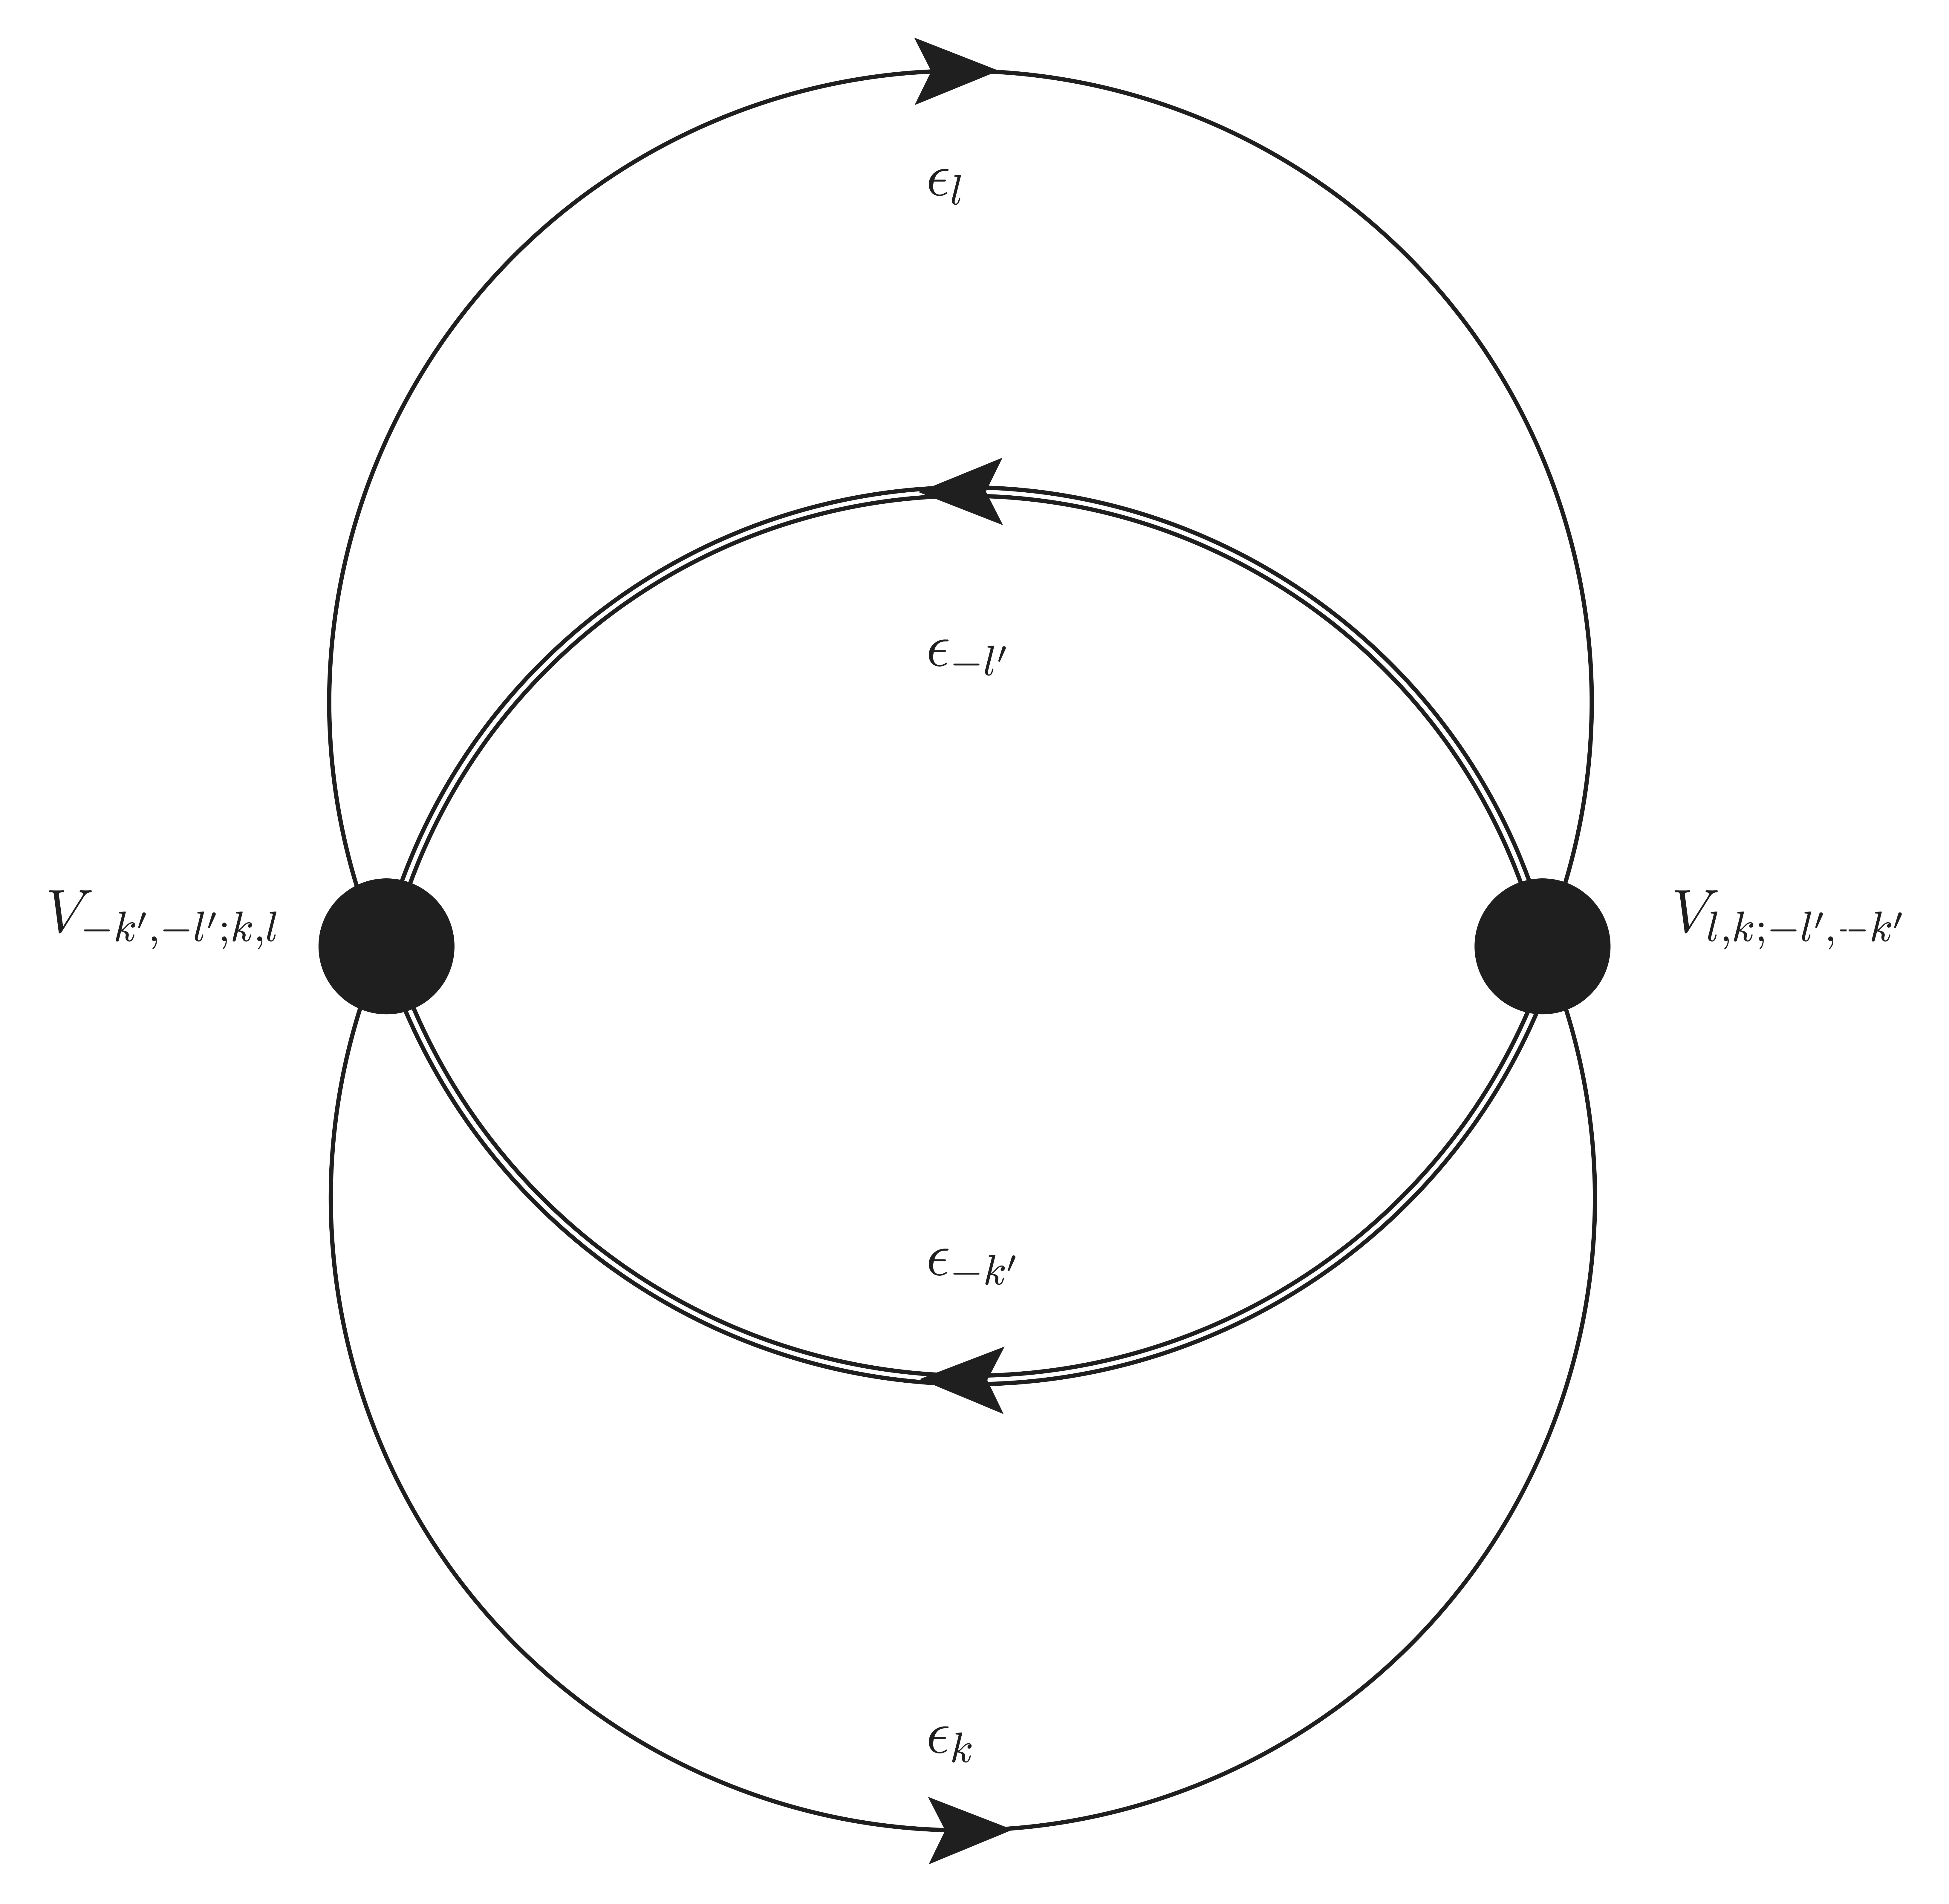
\includegraphics[width=0.65\linewidth,height=\textheight,keepaspectratio]{assets/groundState.png}

\subsubsection{\texorpdfstring{Single-particle state
\(|p,\uparrow\rangle\)}{Single-particle state \textbar p,\textbackslash uparrow\textbackslash rangle}}\label{single-particle-state-puparrowrangle}

\[
\sum_{n}\langle p,\uparrow|\tilde V|n\rangle\frac{1}{\langle p,\uparrow|\tilde H_0|p,\uparrow\rangle-\langle n|\tilde H_0|n\rangle}\langle n|\tilde V|p,\uparrow\rangle
\]

There are two pairs of terms in this case that contribute: terms 3 and
4, and terms 6 and 11 (as for the ground state), but with restrictions

\begin{multline}
\sum_{n}\langle p,\uparrow|V_{p,-l';k,l}a^\dagger_{p,\uparrow}b^{}_{-l',\downarrow}a^{}_{k,\downarrow}a^{}_{l,\uparrow}|n\rangle\frac{1}{\langle p,\uparrow|\tilde H_0|p,\uparrow\rangle-\langle n|\tilde H_0|n\rangle}\langle n|V_{k',l';-k,p}a^\dagger_{k',\uparrow}a^\dagger_{l',\downarrow}b^\dagger_{-k,\downarrow}a^{}_{p,\uparrow}|p,\uparrow\rangle\\
+
\sum_{n}\langle p,\uparrow|V_{-k',-l';k,l\ne p}b^{}_{-k',\uparrow}b^{}_{-l',\downarrow}a^{}_{k,\downarrow}a^{}_{l,\uparrow}|n\rangle\frac{1}{\langle p,\uparrow|\tilde H_0|p,\uparrow\rangle-\langle n|\tilde H_0|n\rangle}\langle n|V_{\tilde k'\ne p,\tilde l';-\tilde k,-\tilde l}a^\dagger_{\tilde k',\uparrow}a^\dagger_{\tilde l',\downarrow}b^\dagger_{-\tilde k,\downarrow}b^\dagger_{-\tilde l,\uparrow}|p,\uparrow\rangle
\end{multline}

\begin{center}\rule{0.5\linewidth}{0.5pt}\end{center}

The first term requires

\[
|n\rangle=|l,\uparrow;k,\downarrow;-l',\downarrow\rangle=a^{\dagger}_{l,\uparrow}a^{\dagger}_{k,\downarrow}b^{\dagger}_{-l',\downarrow}|\Omega\rangle
\quad;\quad \tilde k'=l,\tilde l'=k,\tilde k=l'
\]

The second term requires

\[
|n\rangle=|l\ne p,\uparrow;k,\downarrow;-l',\downarrow;-k',\uparrow;p,\uparrow\rangle=a^{\dagger}_{l\ne p,\uparrow}a^{\dagger}_{k,\downarrow}b^{\dagger}_{-l',\downarrow}b^{\dagger}_{-k',\uparrow}a^{\dagger}_{p,\uparrow}|\Omega\rangle
\quad;\quad \tilde k'=l\ne p,\tilde l'=k,\tilde k=l',\tilde l=k'
\]

When I apply these conditions I finally get

\[
\frac{V_{p,-l';k,l}V_{l,k;-l',p}}{\epsilon_p-\epsilon_k-\epsilon_l+\epsilon_{-l'}} -
\frac{V_{-k',-l';k,l\ne p}V_{l\ne p,k;-l',-k'}}{\epsilon_{l\ne p}+\epsilon_{k}-\epsilon_{-l'}-\epsilon_{-k'}}
\] Notice that the second term is \emph{almost} like the ground state
shift at second order in Equation~\ref{eq-groundStateV2}.

\begin{center}
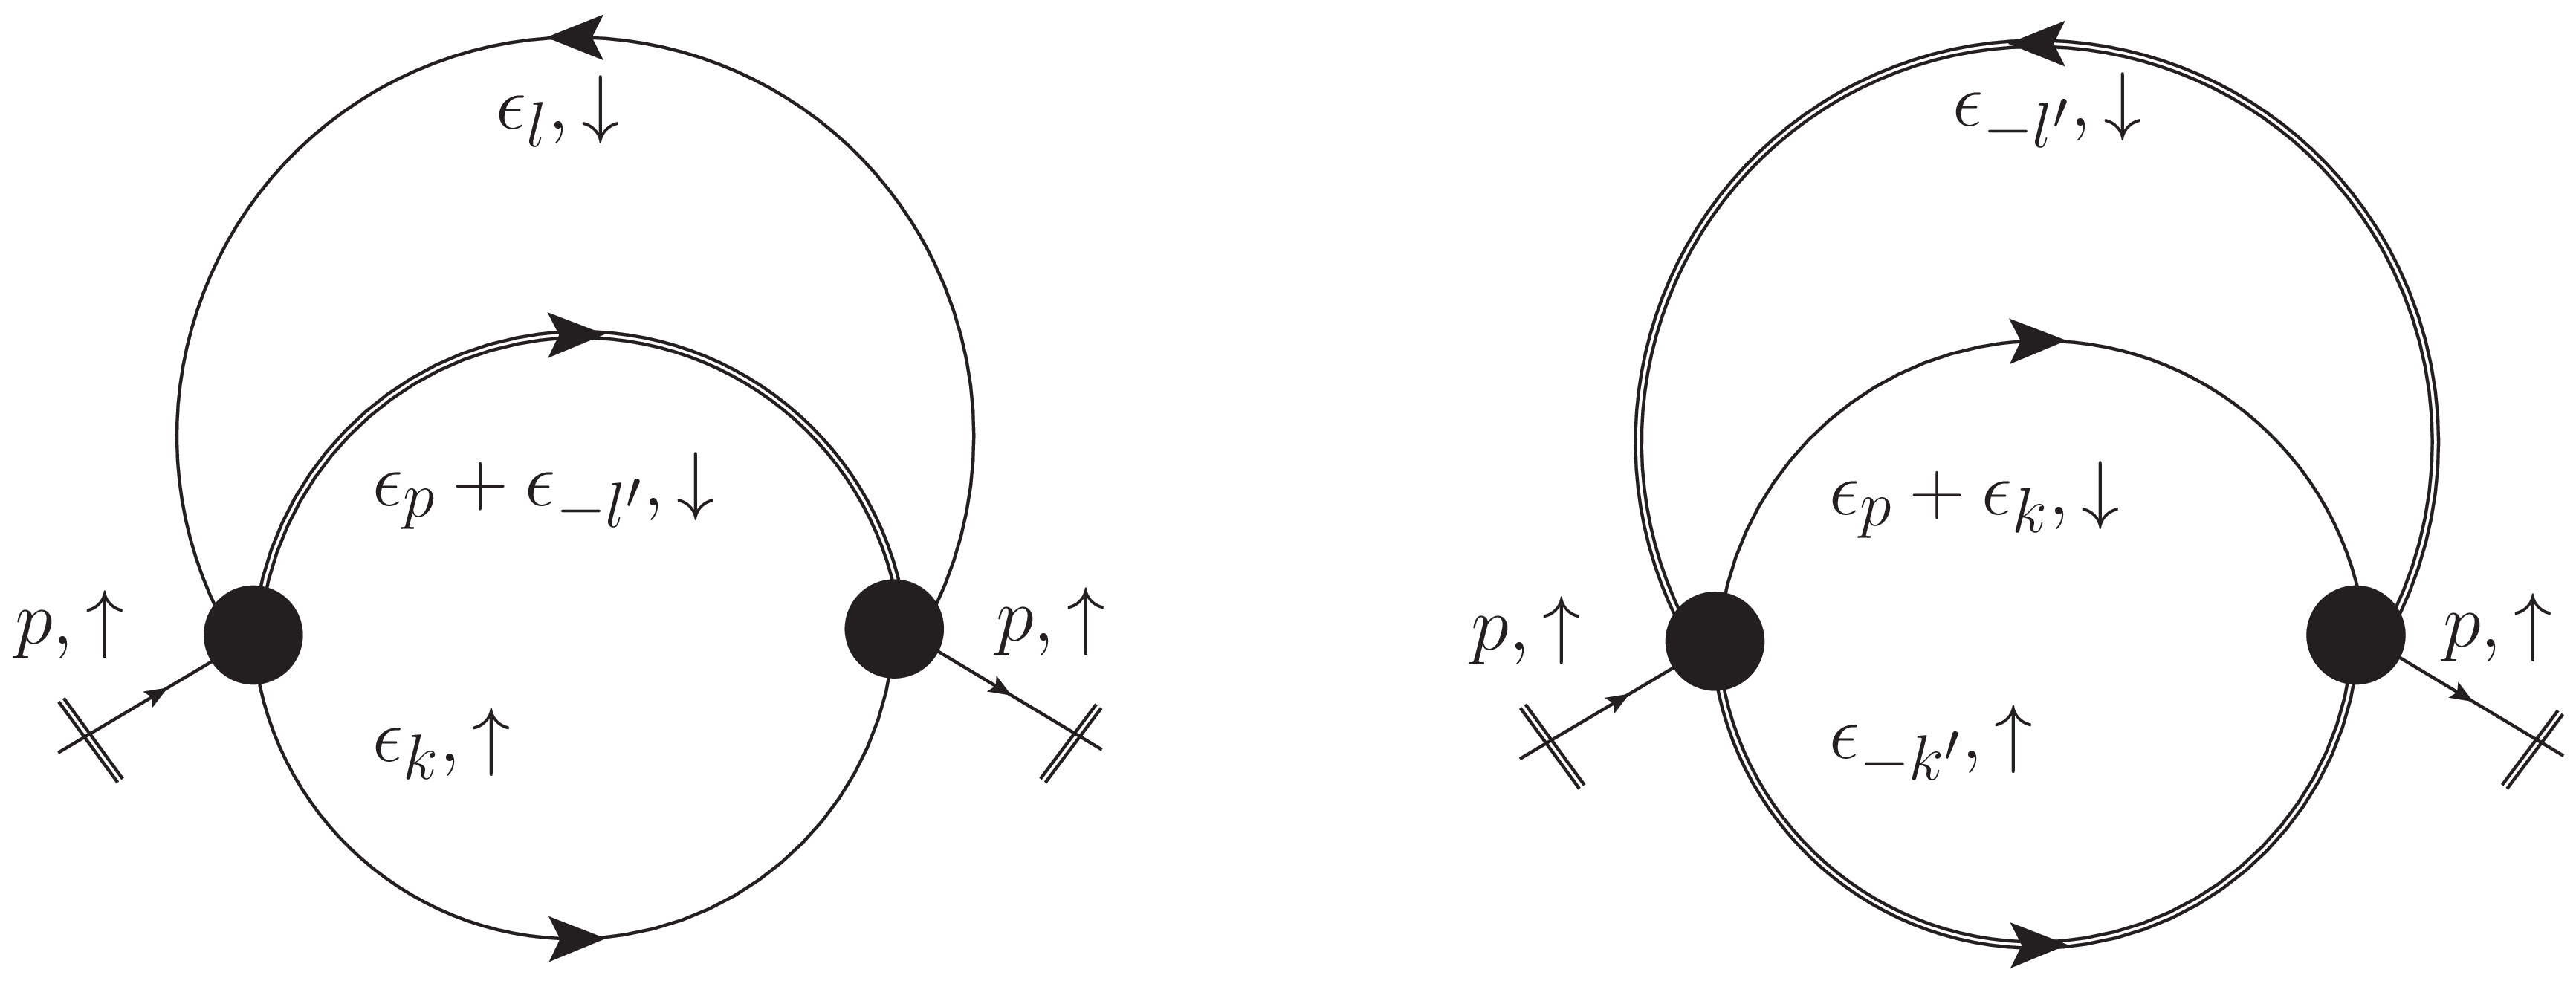
\includegraphics[width=0.8\linewidth,height=\textheight,keepaspectratio]{assets/OrderU2_single.png}
\end{center}

\begin{tcolorbox}[enhanced jigsaw, arc=.35mm, bottomrule=.15mm, bottomtitle=1mm, breakable, colback=white, colbacktitle=quarto-callout-note-color!10!white, colframe=quarto-callout-note-color-frame, coltitle=black, left=2mm, leftrule=.75mm, opacityback=0, opacitybacktitle=0.6, rightrule=.15mm, title=\textcolor{quarto-callout-note-color}{\faInfo}\hspace{0.5em}{Energy difference at \(\mathcal{O}(V^2)\)}, titlerule=0mm, toprule=.15mm, toptitle=1mm]

A little work shows that (I now add the explicit summation symbols) \[
E^{(2)}_{p,s}-E^{(2)}_\Omega=\epsilon_p+\sum_{-l',k,l}\frac{V_{p,-l';k,l}V_{l,k;-l',p}}{\epsilon_p-\epsilon_k-\epsilon_l+\epsilon_{-l'}} +
\sum_{-k',-l',k}\frac{V_{-k',-l';k,p}V_{p,k;-l',-k'}}{\epsilon_{p}+\epsilon_{k}-\epsilon_{-l'}-\epsilon_{-k'}}
\]

\end{tcolorbox}

\subsection{Degenerate perturbation
theory}\label{degenerate-perturbation-theory}

Lin points out a very important fact that I have ignored up to now: the
interesting systems have in the non-interacting limit single-particle
degenerate zero-energy states. If I want to do perturbation theory
properly, I have to perform \emph{degenerate} perturbation theory. So
let's do this now.

I assume there are degenerate single-particle states whose energy
\(\epsilon_d=0\). The systems we are interested in (ie armchair
ribbons), if they have a zero energy, will have a degeneracy of 4 (2 for
spin, and 2 for band). I label these single-particle degenerate states
as \[
c^\dagger_{d,s,+}|0\rangle \equiv a^\dagger_{+d,s}|0\rangle\quad;\quad c^\dagger_{d,s,-}|0\rangle\equiv b^{}_{-d,s}|0\rangle
\] where \(d\) denotes the degenerate state, \(s=\uparrow,\downarrow\),
and the \(\pm\) index denotes the parity of the state\footnote{Lin
  points out correctly that we have full control over the parity of
  these non-interacting states.}.

With this definition I define the half-filled state as before

\begin{equation}\protect\phantomsection\label{eq-groundStateDeg}{
\begin{equation}
|\Omega\rangle=\left(\prod_{-k,s}b_{-k,s}\right)|0\rangle\quad\forall\ \epsilon_{-k}\le 0\ .
\end{equation}
}\end{equation}

Note that \(|\Omega\rangle\) is a spin-singlet positive parity state.

\begin{center}\rule{0.5\linewidth}{0.5pt}\end{center}

Because of these single-particle degenerate states, we now have
\textbf{\emph{16}} \emph{many}-body non-interacting degenerate
states\footnote{Recall that the creation of a hole with spin \(s\),
  \(b^\dagger_{-d,s}\), is equivalent to \textbf{\emph{removing}} a
  particle with spin \(s\), resulting in the system \emph{gaining} spin
  \(-s\).}

\begin{equation}\protect\phantomsection\label{eq-states16}{
\begin{align}
 & b^\dagger_{-d,\uparrow}b^\dagger_{-d,\downarrow}|\Omega\rangle & & & S=0 &&  S_z=0 && Q=-2 && \Pi=+1\\
& b^\dagger_{-d,s}|\Omega\rangle &  & & S=\frac{1}{2} && S_z=\pm\frac{1}{2} && Q=-1 && \Pi=-1\\
& a^\dagger_{d,s}b^\dagger_{-d,\uparrow}b^\dagger_{-d,\downarrow}|\Omega\rangle &  & & S=\frac{1}{2} && S_z=\pm\frac{1}{2} && Q=-1 && \Pi=+1\\
|\Omega\rangle & & a^\dagger_{d,\uparrow}a^\dagger_{d,\downarrow}b^\dagger_{-d,\uparrow}b^\dagger_{-d,\downarrow}|\Omega\rangle & & S=0 && S_z=0 && Q=0 && \Pi=+1\\
a^\dagger_{d,\uparrow}b^\dagger_{-d,\uparrow}|\Omega\rangle & & a^\dagger_{d,\downarrow}b^\dagger_{-d,\downarrow}|\Omega\rangle  & & S=?? && S_z=0 && Q=0 && \Pi=-1\\
a^\dagger_{d,\uparrow}b^\dagger_{-d,\downarrow}|\Omega\rangle & & a^\dagger_{d,\downarrow}b^\dagger_{-d,\uparrow}|\Omega\rangle  & & S=1 && S_z=\pm1 && Q=0 && \Pi=-1\\
& b^\dagger_{-d,s}a^\dagger_{d,\uparrow}a^\dagger_{d,\downarrow}|\Omega\rangle &  & & S=\frac{1}{2} && S_z=\pm\frac{1}{2} && Q=+1 && \Pi=-1\\
& a^\dagger_{d,s}|\Omega\rangle &  & & S=\frac{1}{2} && S_z=\pm\frac{1}{2} && Q=+1 && \Pi=+1\\
& a^\dagger_{d,\uparrow}a^\dagger_{d,\downarrow}|\Omega\rangle & & & S=0 &&  S_z=0 && Q=+2 && \Pi=+1\\
\end{align}
}\end{equation}

All these states have eigenenergy
\(\mathcal{E}_\Omega-\frac{U}{2}\Lambda\), but they have different total
spin \(S\) (if known), spin projection \(S_z\), charge \(Q\), and parity
\(\Pi\) as labelled above. The interaction \(\tilde V\) does not violate
these quantum numbers.

\begin{center}\rule{0.5\linewidth}{0.5pt}\end{center}

\subsubsection{First order (degenerate) perturbation
theory}\label{first-order-degenerate-perturbation-theory}

To perform degenerate perturbation theory at leading order, I need to
diagonalize within the different \(Q,\ S_z\), and \(\Pi\) subspaces. It
is good to refer to Equation~\ref{eq-tildeV}.

\begin{tcolorbox}[enhanced jigsaw, arc=.35mm, bottomrule=.15mm, bottomtitle=1mm, breakable, colback=white, colbacktitle=quarto-callout-note-color!10!white, colframe=quarto-callout-note-color-frame, coltitle=black, left=2mm, leftrule=.75mm, opacityback=0, opacitybacktitle=0.6, rightrule=.15mm, title={\(Q=\pm2\)}, titlerule=0mm, toprule=.15mm, toptitle=1mm]

I start with both \(Q=\pm2\) states because why not. It is trivial to
see that

\begin{align}
& \langle \Omega|b^{}_{-d,\downarrow}b^{}_{-d,\uparrow}\ \tilde V\ b^\dagger_{-d,\uparrow}b^\dagger_{-d,\downarrow}|\Omega\rangle =V_{-d,-d;-d,-d}\\
& \langle \Omega|a^{}_{d,\downarrow}a^{}_{d,\uparrow}\ \tilde V\ a^\dagger_{d,\uparrow}a^\dagger_{d,\downarrow}|\Omega\rangle =V_{d,d;d,d}
\end{align}

I'm willing to bet 5 cents that \(V_{-d,-d;-d,-d}=V_{d,d;d,d}\), which
would mean the shifts for \(Q=\pm 2\) are the same, which is what we
expect!

\end{tcolorbox}

\begin{tcolorbox}[enhanced jigsaw, arc=.35mm, bottomrule=.15mm, bottomtitle=1mm, breakable, colback=white, colbacktitle=quarto-callout-note-color!10!white, colframe=quarto-callout-note-color-frame, coltitle=black, left=2mm, leftrule=.75mm, opacityback=0, opacitybacktitle=0.6, rightrule=.15mm, title={\(Q=-1\)}, titlerule=0mm, toprule=.15mm, toptitle=1mm]

I will just consider \(S_z=\frac{1}{2}\). The \(S_z=-\frac{1}{2}\) gives
the same result. Here is the basis and matrix

\begin{equation}
\left\lvert Q=-1;S_z=\frac{1}{2}\right\rangle=
\begin{pmatrix}
b^\dagger_{-d,\downarrow}\\
a^\dagger_{d,\uparrow}b^\dagger_{-d,\uparrow}b^\dagger_{-d,\downarrow}
\end{pmatrix}
|\Omega\rangle
\quad;\quad \left\langle Q=-1;S_z=\frac{1}{2}\right\rvert\tilde V\left\lvert Q=-1;S_z=\frac{1}{2}\right\rangle=
\begin{bmatrix}
0 & V_{-d,-d;-d,d}\\
V_{d,-d;-d,-d} & V_{-d,-d;-d,-d}-V_{d,-d;-d,d}
\end{bmatrix}
\end{equation}

Now I'm willing to bet 10 cents that \(V_{-d,-d;-d,-d}=V_{d,-d;-d,d}\),
which would mean the matrix becomes

\begin{equation}
\begin{bmatrix}
0 & V_{d,-d;-d,-d}\\
V_{-d,-d;-d,d} & 0
\end{bmatrix}
\end{equation}

If \(V_{d,-d;-d,-d}=V_{-d,-d;-d,d}\) then the diagonalization of this
matrix is trivial. I will confirm this later. Also note that parities
are mixed in this case. The same things happen for the \(Q=+1\) sector.

\textbf{UPDATE: I have numerically confirmed that
\(V_{d,-d;-d,-d}=V_{-d,-d;-d,d}=0\). This means that the parities do NOT
mix and there is no shift at LO.}

\end{tcolorbox}

\begin{center}\rule{0.5\linewidth}{0.5pt}\end{center}

\begin{tcolorbox}[enhanced jigsaw, arc=.35mm, bottomrule=.15mm, bottomtitle=1mm, breakable, colback=white, colbacktitle=quarto-callout-note-color!10!white, colframe=quarto-callout-note-color-frame, coltitle=black, left=2mm, leftrule=.75mm, opacityback=0, opacitybacktitle=0.6, rightrule=.15mm, title={\(Q=0,\ S=0,\ S_z=0,\ \Pi=+1\)}, titlerule=0mm, toprule=.15mm, toptitle=1mm]

Here is the basis and matrix

\begin{equation}
\left\lvert Q=0;S_z=0;\Pi=+1\right\rangle=
\begin{pmatrix}
1\\
a^\dagger_{d,\uparrow}a^\dagger_{d,\downarrow}b^\dagger_{-d,\uparrow}b^\dagger_{-d,\downarrow}
\end{pmatrix}
|\Omega\rangle
\quad;\quad \left\langle  Q=0;S_z=0;\Pi=+1\right\rvert\tilde V\left\lvert  Q=0;S_z=0;\Pi=+1\right\rangle=
\begin{bmatrix}
0 & -V_{-d,-d;d,d}\\
-V_{d,d;-d,-d} & V_{d,d;d,d}+V_{-d,-d;-d,-d}-V_{-d,d;d,-d}-V_{d,-d;-d,d}
\end{bmatrix}
\end{equation}

Again I'm willing to bet 20 cents that
\(V_{d,d;d,d}=V_{-d,-d;-d,-d}=V_{-d,d;d,-d}=V_{d,-d;-d,d}\), which would
mean the matrix becomes

\begin{equation}
\begin{bmatrix}
0 & -V_{-d,-d;d,d}\\
-V_{d,d;-d,-d} & 0
\end{bmatrix}
\end{equation}

If \(V_{d,d;-d,-d}=V_{-d,-d;d,d}\) then the diagonalization of this
matrix is trivial. I will confirm this later.

\end{tcolorbox}

\begin{tcolorbox}[enhanced jigsaw, arc=.35mm, bottomrule=.15mm, bottomtitle=1mm, breakable, colback=white, colbacktitle=quarto-callout-note-color!10!white, colframe=quarto-callout-note-color-frame, coltitle=black, left=2mm, leftrule=.75mm, opacityback=0, opacitybacktitle=0.6, rightrule=.15mm, title={\(Q=0,\ S=??,\ S_z=0,\ \Pi=-1\)}, titlerule=0mm, toprule=.15mm, toptitle=1mm]

Here is the basis and matrix

\begin{equation}
\left\lvert Q=0;S_z=0;\Pi=-1\right\rangle=
\begin{pmatrix}
a^\dagger_{d,\uparrow}b^\dagger_{-d,\uparrow}\\
a^\dagger_{d,\downarrow}b^\dagger_{-d,\downarrow}
\end{pmatrix}
|\Omega\rangle
\quad;\quad \left\langle  Q=0;S_z=0;\Pi=-1\right\rvert\tilde V\left\lvert  Q=0;S_z=0;\Pi=-1\right\rangle=
\begin{bmatrix}
0 & V_{-d,d;-d,d}\\
V_{d,-d;d,-d} & 0
\end{bmatrix}
\end{equation}

Again, if \(V_{-d,d;-d,d}=V_{d,-d;d,-d}\) then the diagonalization of
this matrix is trivial. I will confirm this later.

\end{tcolorbox}

\begin{tcolorbox}[enhanced jigsaw, arc=.35mm, bottomrule=.15mm, bottomtitle=1mm, breakable, colback=white, colbacktitle=quarto-callout-note-color!10!white, colframe=quarto-callout-note-color-frame, coltitle=black, left=2mm, leftrule=.75mm, opacityback=0, opacitybacktitle=0.6, rightrule=.15mm, title={\(Q=0,\ S=1,\ S_z=\pm 1\)}, titlerule=0mm, toprule=.15mm, toptitle=1mm]

Here is the basis and matrix

\begin{equation}
\left\lvert Q=0;S_z=\pm 1;\right\rangle=
\begin{pmatrix}
a^\dagger_{d,\uparrow}b^\dagger_{-d,\downarrow}\\
a^\dagger_{d,\downarrow}b^\dagger_{-d,\uparrow}
\end{pmatrix}
|\Omega\rangle
\quad;\quad \left\langle  Q=0;S_z=\pm 1\right\rvert\tilde V\left\lvert  Q=0;S_z=\pm 1\right\rangle=
\begin{bmatrix}
-V_{d,-d;-d,d} & 0\\
0 & -V_{-d,d;d,-d}
\end{bmatrix}
\end{equation}

I think things are starting to make sense. . .

\end{tcolorbox}

Refer to Equation~\ref{eq-tildeV}

\begin{center}\rule{0.5\linewidth}{0.5pt}\end{center}

\begin{center}
\pandocbounded{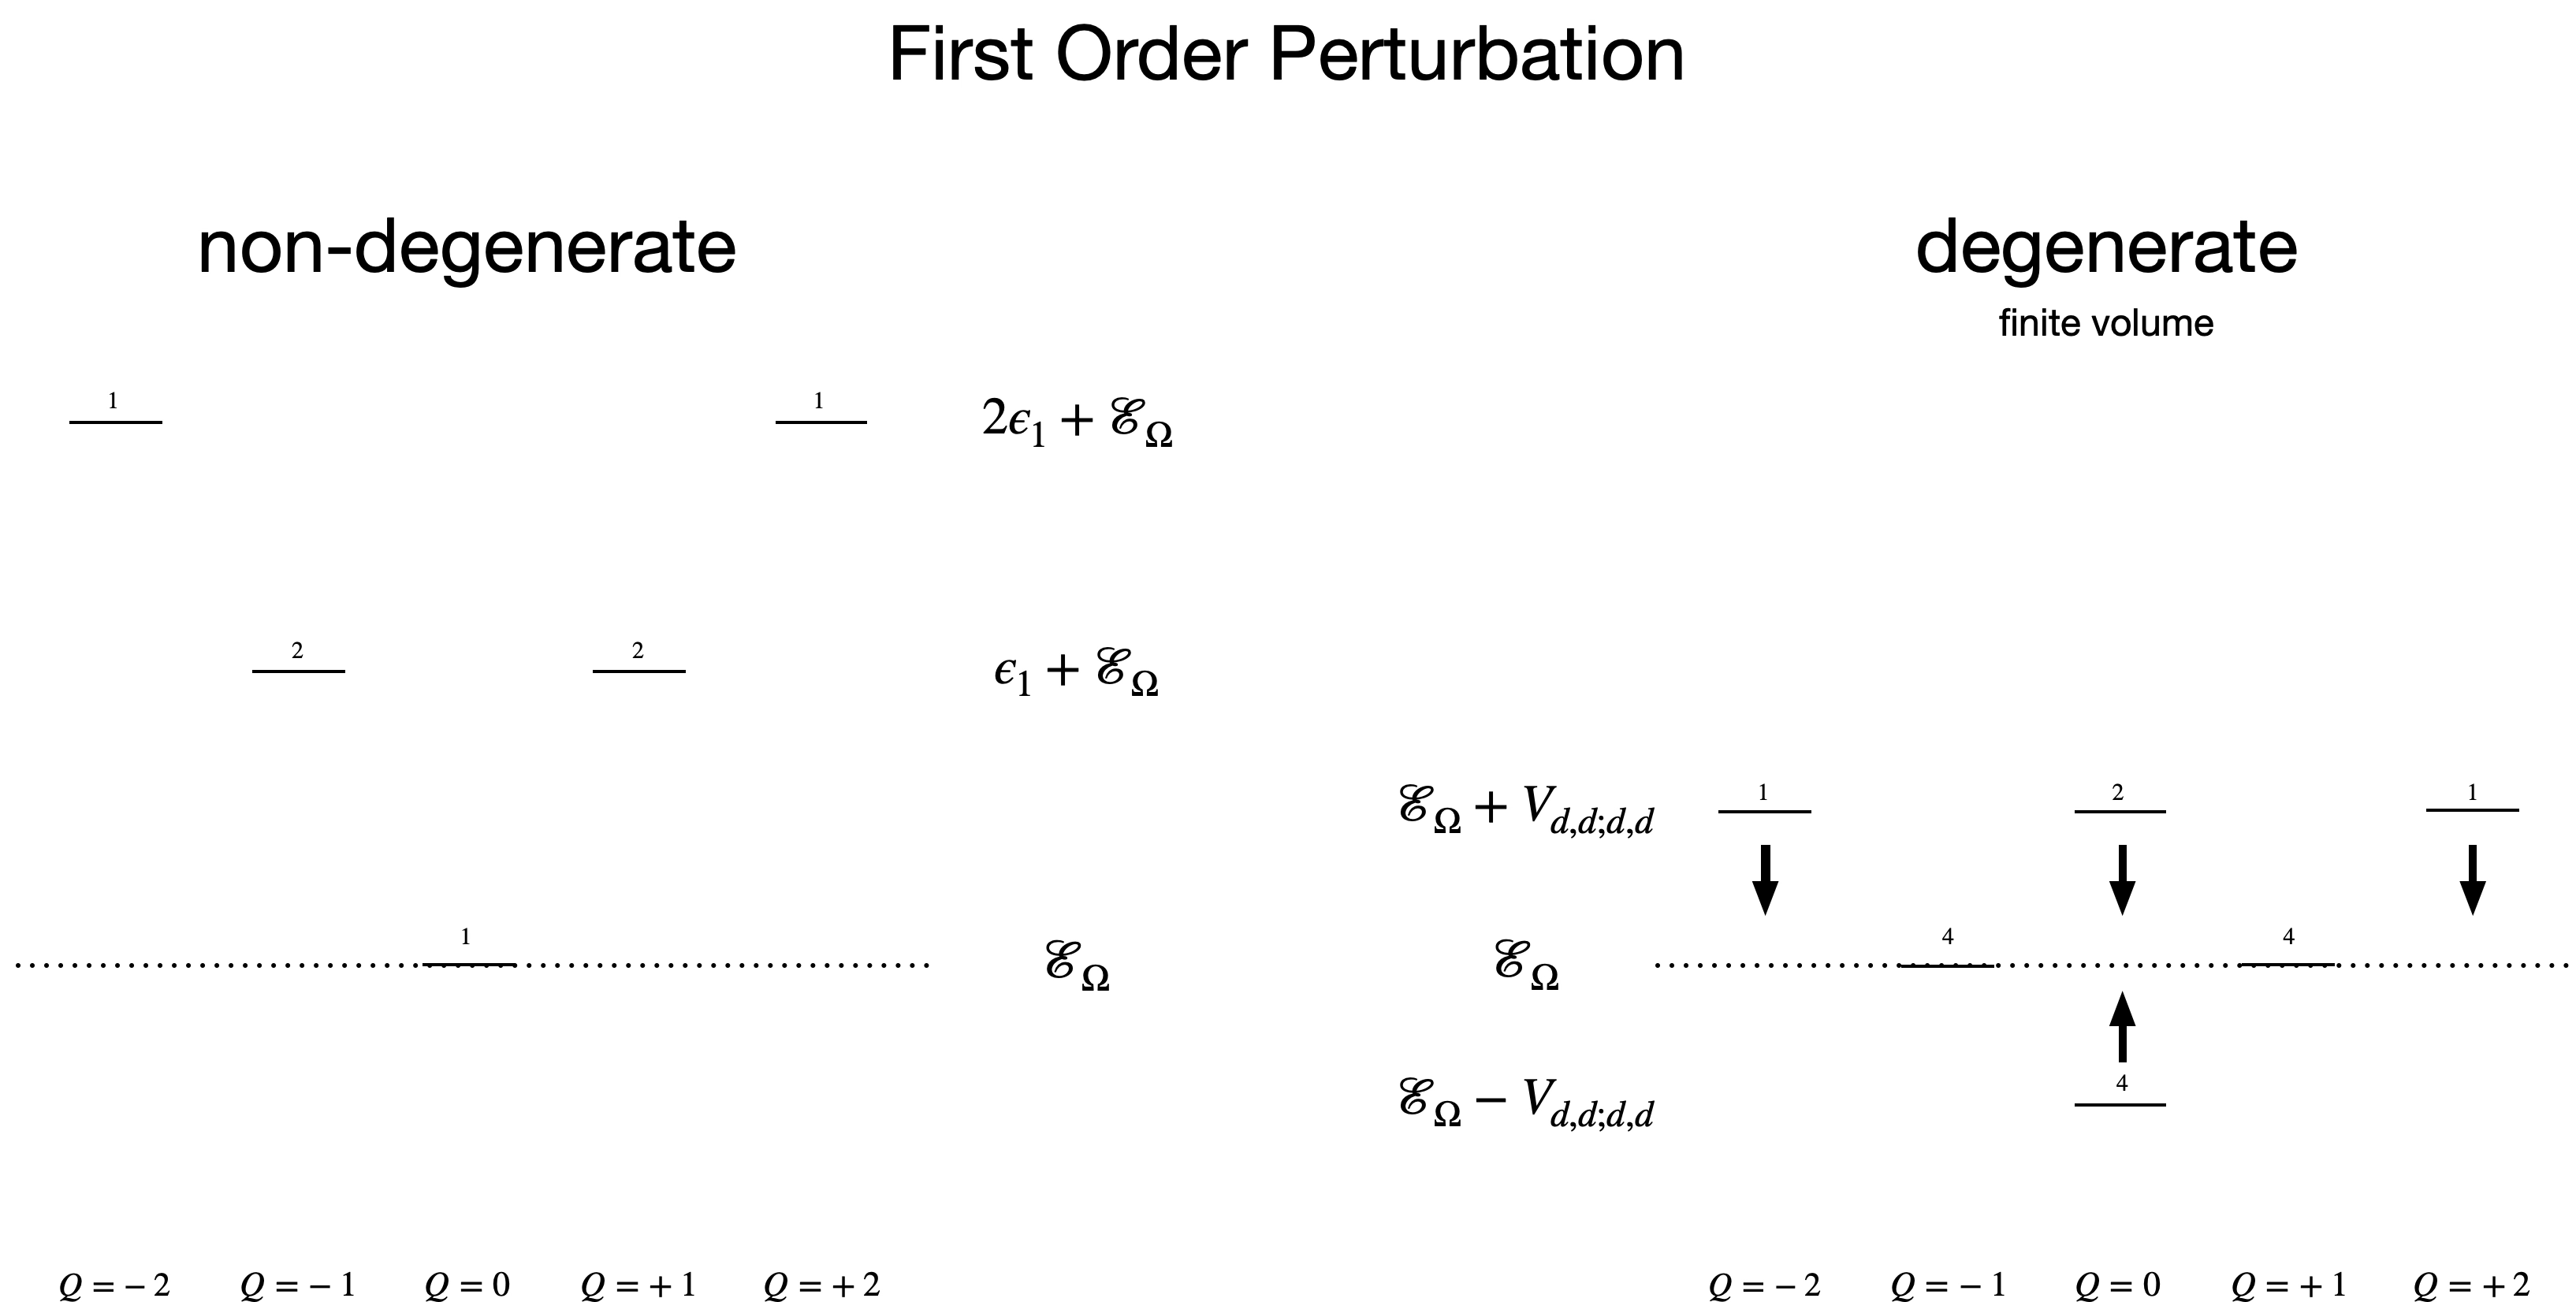
\includegraphics[keepaspectratio]{assets/splittingLO.png}}
\end{center}

\begin{tcolorbox}[enhanced jigsaw, arc=.35mm, bottomrule=.15mm, bottomtitle=1mm, breakable, colback=white, colbacktitle=quarto-callout-warning-color!10!white, colframe=quarto-callout-warning-color-frame, coltitle=black, left=2mm, leftrule=.75mm, opacityback=0, opacitybacktitle=0.6, rightrule=.15mm, title=\textcolor{quarto-callout-warning-color}{\faExclamationTriangle}\hspace{0.5em}{Infinite volume limit \(N_U\to\infty\)}, titlerule=0mm, toprule=.15mm, toptitle=1mm]

For an AGNR with width \(N_W=3m+2\) and number of unit cells \(N_U\) I
have \(\Lambda=N_x/2=N_U\cdot N_W\), where \(N_x\) is the total number
of sites and \(2N_W\) is the number of sites per unit cell. I find that
\begin{equation}
V_{d,d;d,d}=V_{-d,-d;-d,-d}=V_{-d,-d;d,d}=V_{d,d;-d,-d}=V_{-d,d;d,-d}=V_{d,-d;-d,d}=V_{d,-d;d,-d}=V_{-d,d;-d,d}=\frac{1}{4(m+1)N_U}\implies\lim_{N_U\to\infty} V_{d,d;d,d}=0
\end{equation}

\end{tcolorbox}

\begin{center}\rule{0.5\linewidth}{0.5pt}\end{center}

\subsubsection{The new ground state}\label{the-new-ground-state}

So LO perturbation theory shows us that in a finite volume, the ground
state energy gets a shift

\begin{equation}
\mathcal{E}_\Omega-\frac{U\Lambda}{2}\to\mathcal{E}_\Omega-\frac{U\Lambda}{2}-\frac{U}{4(m+1)N_U}\ ,
\end{equation}

where the width of the ribbon is defined as \(N_W=3m+2\).

There are both spin singlet as well as spin triplet eigenstates

\[ \mathcal{E}_\Omega-V_{d,d;d,d} \]

\begin{align}
|\Omega_0,S=0\rangle&=\frac{1}{\sqrt{2}}\left(1+a^\dagger_{d,\uparrow}a^\dagger_{d,\downarrow}b^\dagger_{-d,\uparrow}b^\dagger_{-d,\downarrow}\right)|\Omega\rangle\\
|\Omega,S=1\rangle&=
\begin{cases}
a^\dagger_{d,\uparrow}b^\dagger_{-d,\downarrow}|\Omega\rangle & (S_z=+1)\\
\frac{1}{\sqrt{2}}\left(a^\dagger_{d,\uparrow}b^\dagger_{-d,\uparrow}-a^\dagger_{d,\downarrow}b^\dagger_{-d,\downarrow}\right)|\Omega\rangle & (S_z=0)\\
a^\dagger_{d,\downarrow}b^\dagger_{-d,\uparrow}|\Omega\rangle & (S_z=-1)
\end{cases}
\end{align}

\[ \mathcal{E}_\Omega+V_{d,d;d,d} \]

\begin{align}
|\Omega_1,S=0\rangle&=\frac{1}{\sqrt{2}}\left(1-a^\dagger_{d,\uparrow}a^\dagger_{d,\downarrow}b^\dagger_{-d,\uparrow}b^\dagger_{-d,\downarrow}\right)|\Omega\rangle\\
|\Omega_2,S=0\rangle&=
\frac{1}{\sqrt{2}}\left(a^\dagger_{d,\uparrow}b^\dagger_{-d,\uparrow}+a^\dagger_{d,\downarrow}b^\dagger_{-d,\downarrow}\right)|\Omega\rangle 
\end{align}

where \(|\Omega\rangle\) is defined in Equation~\ref{eq-groundStateDeg}.

\begin{tcolorbox}[enhanced jigsaw, arc=.35mm, bottomrule=.15mm, bottomtitle=1mm, breakable, colback=white, colbacktitle=quarto-callout-important-color!10!white, colframe=quarto-callout-important-color-frame, coltitle=black, left=2mm, leftrule=.75mm, opacityback=0, opacitybacktitle=0.6, rightrule=.15mm, title=\textcolor{quarto-callout-important-color}{\faExclamation}\hspace{0.5em}{Important}, titlerule=0mm, toprule=.15mm, toptitle=1mm]

Again, the LO shift vanishes as \(m\to\infty\) and/or \(N_U\to\infty\).

\end{tcolorbox}

\begin{tcolorbox}[enhanced jigsaw, arc=.35mm, bottomrule=.15mm, bottomtitle=1mm, breakable, colback=white, colbacktitle=quarto-callout-note-color!10!white, colframe=quarto-callout-note-color-frame, coltitle=black, left=2mm, leftrule=.75mm, opacityback=0, opacitybacktitle=0.6, rightrule=.15mm, title=\textcolor{quarto-callout-note-color}{\faInfo}\hspace{0.5em}{Energy difference at \(\mathcal{O}(V)\)}, titlerule=0mm, toprule=.15mm, toptitle=1mm]

\(\therefore\quad\) the energy difference
\(E^{(1)}_{p,s}-E^{(1)}_\Omega=\epsilon_p+\frac{U}{4(m+1)N_U}\)

\end{tcolorbox}

\begin{center}\rule{0.5\linewidth}{0.5pt}\end{center}

\subsubsection{2nd order (degenerate) perturbation
theory}\label{nd-order-degenerate-perturbation-theory}

I want to consider first the singlet ground state case,

\begin{equation}
\sum_{n\ne \pm d} \langle\Omega_0,S=0|\tilde V|n\rangle\frac{1}{\langle\Omega_0,S=0|\tilde H_0|\Omega_0,S=0\rangle-\langle n|\tilde H_0|n\rangle}\langle n|\tilde V|\Omega_0,S=0\rangle
\end{equation}

There are three terms that contribute to this effect\footnote{Actually
  there are four terms, but the cross terms are identical.}. The first
term is

\begin{equation}
\frac{1}{2}\sum_{n\ne \pm d}\langle\Omega|\tilde V|n\rangle\frac{1}{\mathcal{E}_\Omega-\frac{U\Lambda}{2}-\langle n|\tilde H_0|n\rangle}\langle n|\tilde V|\Omega\rangle
\end{equation}

We've done this already in Section~\ref{sec-2ndOrderGroundState}. The
result is similar to Equation~\ref{eq-groundStateV2}, but with some
restrictions on the sums

\begin{equation}
\boxed{
\frac{1}{2}\sum_{n\ne\pm d}\langle\Omega|\tilde V|n\rangle\frac{1}{\langle\Omega|\tilde H_0|\Omega\rangle-\langle n|\tilde H_0|n\rangle}\langle n|\tilde V|\Omega\rangle=
-\frac{1}{2}\sum_{k',l',k,l\ne d}\frac{V_{-k',-l';k,l}V_{l,k;-l',-k'}}{\epsilon_l+\epsilon_k-\epsilon_{-l'}-\epsilon_{-k'}}
}
\end{equation}

The restriction on the sums \(k',l',k,l\) is such that at most three of
these terms can be equal to \(d\), but not all four. In other words the
denominator cannot vanish.

\begin{center}\rule{0.5\linewidth}{0.5pt}\end{center}

The second term is the ``cross'' term,

\begin{equation}
\sum_{n\ne \pm d}\langle\Omega|\tilde V|n\rangle\frac{1}{\mathcal{E}_\Omega-\frac{U\Lambda}{2}-\langle n|\tilde H_0|n\rangle}\langle n|\tilde Va^\dagger_{d,\uparrow}a^\dagger_{d,\downarrow}b^\dagger_{-d,\uparrow}b^\dagger_{-d,\downarrow}|\Omega\rangle
\end{equation}

For this matrix element to be non-vanishing, the \(\tilde V\) on the
left must be term 11 in Equation~\ref{eq-tildeV}. The \(\tilde V\) on
the right can be terms 1, 8, 9, and 16,

\begin{equation}
\langle\Omega|V_{-\kappa',-\lambda',\kappa,\lambda}b_{-\kappa',\uparrow}b_{-\lambda',\downarrow}a_{\kappa,\downarrow}a_{\lambda,\uparrow}|n\rangle\frac{1}{\mathcal{E}_\Omega-\frac{U\Lambda}{2}-\langle n|\tilde H_0|n\rangle}\langle n|
\left\{
\begin{matrix}
V_{k',l';k,l}a^\dagger_{k',\uparrow}a^\dagger_{l',\downarrow}a_{k,\downarrow}a_{l,\uparrow}\\
-V_{-k',l';k,-l}a^\dagger_{l',\downarrow}b^\dagger_{-l,\uparrow}b_{-k',\uparrow}a_{k,\downarrow}\\
-V_{k',-l';-k,l}a^\dagger_{k',\uparrow}b^\dagger_{-k,\downarrow}b_{-l',\downarrow}a_{l,\uparrow}\\
V_{-k',-l';-k,-l}b^\dagger_{-k,\downarrow}b^\dagger_{-l,\uparrow}b_{-k',\uparrow}b_{-l',\downarrow}
\end{matrix}
\right\}
a^\dagger_{d,\uparrow}a^\dagger_{d,\downarrow}b^\dagger_{-d,\uparrow}b^\dagger_{-d,\downarrow}|\Omega\rangle
\end{equation} \begin{equation}
=\langle\Omega|V_{-\kappa',-\lambda',\kappa,\lambda}b_{-\kappa',\uparrow}b_{-\lambda',\downarrow}a_{\kappa,\downarrow}a_{\lambda,\uparrow}|n\rangle\frac{1}{\mathcal{E}_\Omega-\frac{U\Lambda}{2}-\langle n|\tilde H_0|n\rangle}\langle n|
\left\{
\begin{matrix}
V_{k',l';d,d}a^\dagger_{k',\uparrow}a^\dagger_{l',\downarrow}b^\dagger_{-d,\uparrow}b^\dagger_{-d,\downarrow}\\
-V_{-d,l';d,-l}a^\dagger_{l',\downarrow}b^\dagger_{-l,\uparrow}a^\dagger_{d,\uparrow}b^\dagger_{-d,\downarrow}\\
-V_{k',-d;-k,d}a^\dagger_{k',\uparrow}b^\dagger_{-k,\downarrow}a^\dagger_{d,\downarrow}b^\dagger_{-d,\uparrow}\\
-V_{-d,-d;-k,-l}b^\dagger_{-k,\downarrow}b^\dagger_{-l,\uparrow}a^\dagger_{d,\uparrow}a^\dagger_{d,\downarrow}
\end{matrix}
\right\}
|\Omega\rangle
\end{equation} \begin{equation}
=\langle\Omega|V_{-\kappa',-\lambda',\kappa,\lambda}b_{-\kappa',\uparrow}b_{-\lambda',\downarrow}a_{\kappa,\downarrow}a_{\lambda,\uparrow}|n\rangle\frac{1}{\mathcal{E}_\Omega-\frac{U\Lambda}{2}-\langle n|\tilde H_0|n\rangle}\langle n|
\left\{
\begin{matrix}
-V_{k',l';d,d}a^\dagger_{k',\uparrow}a^\dagger_{l',\downarrow}b^\dagger_{-d,\downarrow}b^\dagger_{-d,\uparrow}\\
+V_{-d,l';d,-l}a^\dagger_{d,\uparrow}a^\dagger_{l',\downarrow}b^\dagger_{-d,\downarrow}b^\dagger_{-l,\uparrow}\\
+V_{k',-d;-k,d}a^\dagger_{k',\uparrow}a^\dagger_{d,\downarrow}b^\dagger_{-k,\downarrow}b^\dagger_{-d,\uparrow}\\
-V_{-d,-d;-k,-l}a^\dagger_{d,\uparrow}a^\dagger_{d,\downarrow}b^\dagger_{-k,\downarrow}b^\dagger_{-l,\uparrow}
\end{matrix}
\right\}
|\Omega\rangle
\end{equation}

\begin{center}\rule{0.5\linewidth}{0.5pt}\end{center}

Therefore the ``cross'' term is\footnote{Recall that
  \(\epsilon_{-l}=-\epsilon_{l}\) and \(\epsilon_{-d}=\epsilon_{d}=0\).}

\[
\boxed{
\begin{align}
&\sum_{n\ne \pm d}\langle\Omega|\tilde V|n\rangle\frac{1}{\mathcal{E}_\Omega-\frac{U\Lambda}{2}-\langle n|\tilde H_0|n\rangle}\langle n|\tilde Va^\dagger_{d,\uparrow}a^\dagger_{d,\downarrow}b^\dagger_{-d,\uparrow}b^\dagger_{-d,\downarrow}|\Omega\rangle\\
&=-\sum_{k',l'}\frac{V_{-d,-d;l',k'}V_{k',l';d,d}}{-\epsilon_{l'}-\epsilon_{k'}}
+\sum_{l',l}\frac{V_{-l,-d;l',d}V_{-d,l';d,-l}}{\epsilon_{-l}-\epsilon_{l'}}
+\sum_{k',k}\frac{V_{-d,-k;d,k'}V_{k',-d;-k,d}}{\epsilon_{-k}-\epsilon_{k'}}
-\sum_{k,l}\frac{V_{-l,-k;d,d}V_{-d,-d;-k,-l}}{\epsilon_{-l}+\epsilon_{-k}}
\end{align}
}
\]

The restrictions on the sums are such that the denominators cannot
vanish.

The final term is

\begin{equation}
\frac{1}{2}\sum_{n\ne \pm d}\langle\Omega|b_{-d,\downarrow}b_{-d,\uparrow}a_{d,\downarrow}a_{d,\uparrow}\tilde V|n\rangle\frac{1}{\mathcal{E}_\Omega-\frac{U\Lambda}{2}-\langle n|\tilde H_0|n\rangle}\langle n|\tilde Va^\dagger_{d,\uparrow}a^\dagger_{d,\downarrow}b^\dagger_{-d,\uparrow}b^\dagger_{-d,\downarrow}|\Omega\rangle
\end{equation}

Unfortunately there are a lot of terms in Equation~\ref{eq-tildeV} that
can contribute. They are listed here:

{\def\LTcaptype{none} % do not increment counter
\begin{longtable}[]{@{}cc@{}}
\toprule\noalign{}
left \(\tilde V\) & right \(\tilde V\) \\
\midrule\noalign{}
\endhead
\bottomrule\noalign{}
\endlastfoot
2 & 5 \\
3 & 4 \\
7 & 10 \\
12 & 15 \\
13 & 14 \\
\end{longtable}
}

{\def\LTcaptype{none} % do not increment counter
\begin{longtable}[]{@{}cc@{}}
\toprule\noalign{}
left \(\tilde V\) & right \(\tilde V\) \\
\midrule\noalign{}
\endhead
\bottomrule\noalign{}
\endlastfoot
1 & 1 \\
11 & 6 \\
16 & 16 \\
8 & 8 \\
9 & 9 \\
\end{longtable}
}

{\def\LTcaptype{none} % do not increment counter
\begin{longtable}[]{@{}cc@{}}
\toprule\noalign{}
left \(\tilde V\) & right \(\tilde V\) \\
\midrule\noalign{}
\endhead
\bottomrule\noalign{}
\endlastfoot
5 & 2 \\
4 & 3 \\
10 & 7 \\
15 & 12 \\
14 & 13 \\
\end{longtable}
}

{\def\LTcaptype{none} % do not increment counter
\begin{longtable}[]{@{}cc@{}}
\toprule\noalign{}
left \(\tilde V\) & right \(\tilde V\) \\
\midrule\noalign{}
\endhead
\bottomrule\noalign{}
\endlastfoot
5 & 12 \\
4 & 13 \\
15 & 2 \\
14 & 3 \\
\end{longtable}
}

\begin{center}\rule{0.5\linewidth}{0.5pt}\end{center}

I will work out an explict calculation for the \((2,5)\) and \((5,2)\)
pairs. We have in this case

\begin{equation}
\frac{1}{2}\sum_{n\ne \pm d}\langle\Omega|b_{-d,\downarrow}b_{-d,\uparrow}a_{d,\downarrow}a_{d,\uparrow}
\left\{
\begin{matrix}
-V_{\kappa',\lambda';\kappa,-\lambda}a^\dagger_{\kappa',\uparrow}a^\dagger_{\lambda',\downarrow}b^\dagger_{-\lambda,\uparrow}a_{\kappa,\downarrow}\\
-V_{-\kappa',\lambda';\kappa,\lambda}a^\dagger_{\lambda',\downarrow}b_{-\kappa',\uparrow}a_{\kappa,\downarrow}a_{\lambda,\uparrow}
\end{matrix}
\right\}
|n\rangle\frac{1}{\mathcal{E}_\Omega-\frac{U\Lambda}{2}-\langle n|\tilde H_0|n\rangle}\langle n|\left\{
\begin{matrix}
-V_{-k',l';k,l}a^\dagger_{l',\downarrow}b_{-k',\uparrow}a_{k,\downarrow}a_{l,\uparrow}\\
-V_{k',l';k,-l}a^\dagger_{k',\uparrow}a^\dagger_{l',\downarrow}b^\dagger_{-l,\uparrow}a_{k,\downarrow}
\end{matrix}
\right\}
a^\dagger_{d,\uparrow}a^\dagger_{d,\downarrow}b^\dagger_{-d,\uparrow}b^\dagger_{-d,\downarrow}|\Omega\rangle
\end{equation}

The top pair corresponds to \((2,5)\), and the bottom pair \((5,2)\). An
intermediate step gives

\begin{equation}
\frac{1}{2}\sum_{n\ne \pm d}\langle\Omega|
\left\{
\begin{matrix}
-V_{d,d;\kappa,-d}b_{-d,\downarrow}a_{\kappa,\downarrow}\\
+V_{-\kappa',d;\kappa,\lambda}b_{-d,\downarrow}b_{-d,\uparrow}a_{d,\uparrow}b_{-\kappa',\uparrow}a_{\kappa,\downarrow}a_{\lambda,\uparrow}
\end{matrix}
\right\}
|n\rangle\frac{1}{\mathcal{E}_\Omega-\frac{U\Lambda}{2}-\langle n|\tilde H_0|n\rangle}\langle n|\left\{
\begin{matrix}
-V_{-d,l';d,d}a^\dagger_{l',\downarrow}b^\dagger_{-d,\downarrow}\\
+V_{k',l';d,-l}a^\dagger_{k',\uparrow}a^\dagger_{l',\downarrow}b^\dagger_{-l,\uparrow}a^\dagger_{d,\uparrow}b^\dagger_{-d,\uparrow}b^\dagger_{-d,\downarrow}
\end{matrix}
\right\}
|\Omega\rangle
\end{equation}

The top case is non-vanishing when
\(|n\rangle=a^\dagger_{l',\downarrow}b^\dagger_{-d,\downarrow}|\Omega\rangle\),
while the bottom case is non-vanishing when
\(|n\rangle=a^\dagger_{k',\uparrow}a^\dagger_{l',\downarrow}b^\dagger_{-l,\uparrow}a^\dagger_{d,\uparrow}b^\dagger_{-d,\uparrow}b^\dagger_{-d,\downarrow}|\Omega\rangle\)
and \(k'\ne d\) and \(l\ne d\).

This results in two terms\footnote{It might be that some of these matrix
  elements vanish. Need to check --T.L.} \footnote{Lin has proven that
  \(V_{\pm d,\pm d;\pm d,i}=0\ \forall i\ne\pm d\).}

\begin{equation}
\frac{1}{2}\sum_{l'\ne d}\frac{V_{d,d;l',-d}V_{-d,l';d,d}}{-\epsilon_{l'}}
+
\frac{1}{2}\sum_{k',l\ne d, l'}\frac{V_{-l,d;l',k'}V_{k',l';d,-l}}{\epsilon_{-l}-\epsilon_{k'}-\epsilon_{l'}}
\quad (2,5),\ (5,2)\ \operatorname{pairs}
\end{equation}

Things are getting complicated. The \((11,6)\) pair can be done without
much thinking

\begin{equation}
\frac{1}{2}\sum_{k',l',k,l\ne d}\frac{V_{-k',-l';k,l}V_{l,k;-l',-k'}}{\epsilon_{-k'}+\epsilon_{-l'}-\epsilon_k-\epsilon_l}\quad (11,6)\ \operatorname{pair}
\end{equation}

Here \emph{none} of the indices can be equal to \(d\)

\begin{center}\rule{0.5\linewidth}{0.5pt}\end{center}

After inspection, the \((3,4)\) and \((4,3)\) terms are identical to the
\((2,5)\) and \((5,2)\) terms. So I won't write these terms.

Now I consider the \((7,10)\) and \((10,7)\) terms

\begin{equation}
\frac{1}{2}\sum_{n\ne \pm d}\langle\Omega|b_{-d,\downarrow}b_{-d,\uparrow}a_{d,\downarrow}a_{d,\uparrow}
\left\{
\begin{matrix}
V_{\kappa',-\lambda';\kappa,-\lambda}a^\dagger_{\kappa',\uparrow}b^\dagger_{-\lambda,\uparrow}b_{-\lambda',\downarrow}a_{\kappa,\downarrow}\\
V_{-\kappa',\lambda';-\kappa,\lambda}a^\dagger_{\lambda',\downarrow}b^\dagger_{-\kappa,\downarrow}b_{-\kappa',\uparrow}a_{\lambda,\uparrow}
\end{matrix}
\right\}
|n\rangle\frac{1}{\mathcal{E}_\Omega-\frac{U\Lambda}{2}-\langle n|\tilde H_0|n\rangle}\langle n|\left\{
\begin{matrix}
V_{-k',l';-k,l}a^\dagger_{l',\downarrow}b^\dagger_{-k,\downarrow}b_{-k',\uparrow}a_{l,\uparrow}\\
V_{k',-l';k,-l}a^\dagger_{k',\uparrow}b^\dagger_{-l,\uparrow}b_{-l',\downarrow}a_{k,\downarrow}
\end{matrix}
\right\}
a^\dagger_{d,\uparrow}a^\dagger_{d,\downarrow}b^\dagger_{-d,\uparrow}b^\dagger_{-d,\downarrow}|\Omega\rangle
\end{equation}

\begin{equation}
=\frac{1}{2}\sum_{n\ne \pm d}\langle\Omega|
\left\{
\begin{matrix}
-V_{d,-\lambda';\kappa,-d}b_{-d,\downarrow}a_{d,\downarrow}b_{-\lambda',\downarrow}a_{\kappa,\downarrow}\\
-V_{-\kappa',d;-d,\lambda}b_{-d,\uparrow}a_{d,\uparrow}b_{-\kappa',\uparrow}a_{\lambda,\uparrow}
\end{matrix}
\right\}
|n\rangle\frac{1}{\mathcal{E}_\Omega-\frac{U\Lambda}{2}-\langle n|\tilde H_0|n\rangle}\langle n|\left\{
\begin{matrix}
-V_{-d,l';-k,d}a^\dagger_{l',\downarrow}b^\dagger_{-k,\downarrow}a^\dagger_{d,\downarrow}b^\dagger_{-d,\downarrow}\\
-V_{k',-d;d,-l}a^\dagger_{k',\uparrow}b^\dagger_{-l,\uparrow}a^\dagger_{d,\uparrow}b^\dagger_{-d,\uparrow}
\end{matrix}
\right\}
|\Omega\rangle
\end{equation}

\begin{equation}
=\frac{1}{2}\sum_{l',k\ne d}\frac{V_{d,-k;l',-d}V_{-d,l';-k,d}}{\epsilon_{-k}-\epsilon_{l'}}
+
\frac{1}{2}\sum_{k',l\ne d}\frac{V_{-l,d;-d,k'}V_{k',-d;d,-l}}{\epsilon_{-l}-\epsilon_{k'}}
\quad (7,10),\ (10,7)\ \operatorname{pairs}
\end{equation}

Now Lin predicts that this expression is the result of the (8,8) and
(9,9) pairs as well. I'm very sure that he is correct, but I'll check it
as well,

\begin{equation}
\frac{1}{2}\sum_{n\ne \pm d}\langle\Omega|b_{-d,\downarrow}b_{-d,\uparrow}a_{d,\downarrow}a_{d,\uparrow}
\left\{
\begin{matrix}
-V_{-\kappa',\lambda';\kappa,-\lambda}a^\dagger_{\lambda',\downarrow}b^\dagger_{-\lambda,\uparrow}b_{-\kappa',\uparrow}a_{\kappa,\downarrow}\\
-V_{\kappa',-\lambda';-\kappa,\lambda}a^\dagger_{\kappa',\uparrow}b^\dagger_{-\kappa,\downarrow}b_{-\lambda',\downarrow}a_{\lambda,\uparrow}
\end{matrix}
\right\}
|n\rangle\frac{1}{\mathcal{E}_\Omega-\frac{U\Lambda}{2}-\langle n|\tilde H_0|n\rangle}\langle n|\left\{
\begin{matrix}
-V_{-k',l';k,-l}a^\dagger_{l',\downarrow}b^\dagger_{-l,\uparrow}b_{-k',\uparrow}a_{k,\downarrow}\\
-V_{k',-l';-k,l}a^\dagger_{k',\uparrow}b^\dagger_{-k,\downarrow}b_{-l',\downarrow}a_{l,\uparrow}
\end{matrix}
\right\}
a^\dagger_{d,\uparrow}a^\dagger_{d,\downarrow}b^\dagger_{-d,\uparrow}b^\dagger_{-d,\downarrow}|\Omega\rangle
\end{equation}

\begin{equation}
=\frac{1}{2}\sum_{n\ne \pm d}\langle\Omega|
\left\{
\begin{matrix}
-V_{-\kappa',d;\kappa,-d}b_{-d,\downarrow}a_{d,\uparrow}b_{-\kappa',\uparrow}a_{\kappa,\downarrow}\\
-V_{d,-\lambda';-d,\lambda}b_{-d,\uparrow}a_{d,\downarrow}b_{-\lambda',\downarrow}a_{\lambda,\uparrow}
\end{matrix}
\right\}
|n\rangle\frac{1}{\mathcal{E}_\Omega-\frac{U\Lambda}{2}-\langle n|\tilde H_0|n\rangle}\langle n|\left\{
\begin{matrix}
-V_{-d,l';d,-l}a^\dagger_{l',\downarrow}b^\dagger_{-l,\uparrow}a^\dagger_{d,\uparrow}b^\dagger_{-d,\downarrow}\\
-V_{k',-d;-k,d}a^\dagger_{k',\uparrow}b^\dagger_{-k,\downarrow}a^\dagger_{d,\downarrow}b^\dagger_{-d,\uparrow}
\end{matrix}
\right\}
|\Omega\rangle
\end{equation}

\begin{equation}
=\frac{1}{2}\sum_{l',l\ne d}\frac{V_{-l,d;l',-d}V_{-d,l';d,-l}}{\epsilon_{-l}-\epsilon_{l'}}
+
\frac{1}{2}\sum_{k',k\ne d}\frac{V_{d,-k;-d,k'}V_{k',-d;-k,d}}{\epsilon_{-k}-\epsilon_{k'}}
\quad (8,8),\ (9,9)\ \operatorname{pairs}
\end{equation}

\begin{center}\rule{0.5\linewidth}{0.5pt}\end{center}

Now the (12,15) and (15,12) terms

\begin{equation}
\frac{1}{2}\sum_{n\ne \pm d}\langle\Omega|b_{-d,\downarrow}b_{-d,\uparrow}a_{d,\downarrow}a_{d,\uparrow}
\left\{
\begin{matrix}
V_{\kappa',-\lambda';-\kappa,-\lambda}a^\dagger_{\kappa',\uparrow}b^\dagger_{-\kappa,\downarrow}b^\dagger_{-\lambda,\uparrow}b_{-\lambda',\downarrow}\\
V_{-\kappa',-\lambda';-\kappa,\lambda}b^\dagger_{-\kappa,\downarrow}b_{-\kappa',\uparrow}b_{-\lambda',\downarrow}a_{\lambda,\uparrow}
\end{matrix}
\right\}
|n\rangle\frac{1}{\mathcal{E}_\Omega-\frac{U\Lambda}{2}-\langle n|\tilde H_0|n\rangle}\langle n|\left\{
\begin{matrix}
V_{-k',-l';-k,l}b^\dagger_{-k,\downarrow}b_{-k',\uparrow}b_{-l',\downarrow}a_{l,\uparrow}\\
V_{k',-l';-k,-l}a^\dagger_{k',\uparrow}b^\dagger_{-k,\downarrow}b^\dagger_{-l,\uparrow}b_{-l',\downarrow}
\end{matrix}
\right\}
a^\dagger_{d,\uparrow}a^\dagger_{d,\downarrow}b^\dagger_{-d,\uparrow}b^\dagger_{-d,\downarrow}|\Omega\rangle
\end{equation}

\begin{equation}
=\frac{1}{2}\sum_{n\ne \pm d}\langle\Omega|
\left\{
\begin{matrix}
-V_{d,-\lambda';-d,-d}a_{d,\downarrow}b_{-\lambda',\downarrow}\\
-V_{-\kappa',-\lambda';-d,\lambda}b_{-d,\uparrow}a_{d,\downarrow}a_{d,\uparrow}b_{-\kappa',\uparrow}b_{-\lambda',\downarrow}a_{\lambda,\uparrow}
\end{matrix}
\right\}
|n\rangle\frac{1}{\mathcal{E}_\Omega-\frac{U\Lambda}{2}-\langle n|\tilde H_0|n\rangle}\langle n|\left\{
\begin{matrix}
-V_{-d,-d;-k,d}b^\dagger_{-k,\downarrow}a^\dagger_{d,\downarrow}\\
-V_{k',-d;-k,-l}a^\dagger_{k',\uparrow}b^\dagger_{-k,\downarrow}b^\dagger_{-l,\uparrow}a^\dagger_{d,\uparrow}a^\dagger_{d,\downarrow}b^\dagger_{-d,\uparrow}
\end{matrix}
\right\}
|\Omega\rangle
\end{equation}

\begin{equation}
=\frac{1}{2}\sum_{k,l\ne d}\frac{V_{d,-k;-d,-d}V_{-d,-d;-k,d}}{\epsilon_{-k}}
+
\frac{1}{2}\sum_{k',l\ne d,k}\frac{V_{-l,-k;-d,k'}V_{k',-d;-k,-l}}{\epsilon_{-k}+\epsilon_{-l}-\epsilon_{k'}}
\quad (12,15),\ (15,12)\ \operatorname{pairs}
\end{equation}

Thanks to Lin we know that the first term vanishes since
\(V_{\pm d,\pm d;\pm d,i}=0\ \forall\  i\ne \pm d\).

Ok, by simple inspection (it must be true!!!) we can see that the
(13,14) and (14,13) pairs give the same result as above. So I won't
write them down.

The final pairs (1,1) and (16,16) can be done by inspection

\begin{equation}
\frac{1}{2}\sum_{k,l\ne d}\frac{V_{d,d;k,l}V_{l,k;d,d}}{-\epsilon_{k}-\epsilon_{l}}
+
\frac{1}{2}\sum_{k,l\ne d}\frac{V_{-d,-d;-k,-l}V_{-l,-k;-d,-d}}{\epsilon_{-k}+\epsilon_{-l}}
\quad (1,1),\ (16,16)\ \operatorname{pairs}
\end{equation}

\begin{center}\rule{0.5\linewidth}{0.5pt}\end{center}

I will just write out the remaining pairs:

\begin{itemize}
\tightlist
\item
  \((5,12)\) pair
\end{itemize}

\begin{equation}
-\frac{1}{2}\frac{V_{-d,d,\kappa ,\lambda }^2}{-\epsilon _{\kappa }-\epsilon _{\lambda }}
\end{equation}

\begin{itemize}
\tightlist
\item
  \((4,13)\) pair
\end{itemize}

\begin{equation}
-\frac{1}{2}\frac{V_{-d,d,\kappa ,\lambda }^2}{-\epsilon _{\kappa }-\epsilon _{\lambda }}
\end{equation}

\begin{itemize}
\tightlist
\item
  \((15,2)\) pair
\end{itemize}

\begin{equation}
-\frac{1}{2}\frac{V_{-d,d,\kappa ,\lambda }^2}{-\epsilon _{\kappa }-\epsilon _{\lambda }}
\end{equation}

\begin{itemize}
\tightlist
\item
  \((13,3)\) pair
\end{itemize}

\begin{equation}
-\frac{1}{2}\frac{V_{-d,d,\kappa ,\lambda }^2}{-\epsilon _{\kappa }-\epsilon _{\lambda }}
\end{equation}

\begin{center}\rule{0.5\linewidth}{0.5pt}\end{center}

I will now collect all terms for the singlet ground state shift

\begin{tcolorbox}[enhanced jigsaw, arc=.35mm, bottomrule=.15mm, bottomtitle=1mm, breakable, colback=white, colbacktitle=quarto-callout-note-color!10!white, colframe=quarto-callout-note-color-frame, coltitle=black, left=2mm, leftrule=.75mm, opacityback=0, opacitybacktitle=0.6, rightrule=.15mm, title=\textcolor{quarto-callout-note-color}{\faInfo}\hspace{0.5em}{Spin singlet 2nd-order shift}, titlerule=0mm, toprule=.15mm, toptitle=1mm]

\begin{equation}
\boxed{
-2\sum_{k,l,m\ne d}\frac{V_{k,l;m,d}V_{d,m;l,k}}{\epsilon_{l}+\epsilon_{k}+\epsilon_m}
-2\sum_{k,l,m\ne d}\frac{V_{k,l;m,-d}V_{-d,m;l,k}}{\epsilon_{l}+\epsilon_{k}+\epsilon_m}
-\sum_{k,l,m,p\ne d}\frac{V_{k,l;m,p}V_{p,m;l,k}}{\epsilon_{k}+\epsilon_{l}+\epsilon_m+\epsilon_p}
-6\sum_{k,l\ne d}\frac{V_{d,d;k,l}V_{l,k;d,d}}{\epsilon_{k}+\epsilon_{l}}
}
\end{equation}

None of the indices can be equal to \(d\).

\end{tcolorbox}

A lot of symmetries was used to obtain this compact
expression!\footnote{I hope it's correct!}

So this was for the state
\(|\Omega_0,S=0\rangle=\frac{1}{\sqrt{2}}\left(1+a^\dagger_{d,\uparrow}a^\dagger_{d,\downarrow}b^\dagger_{-d,\uparrow}b^\dagger_{-d,\downarrow}\right)|\Omega\rangle\).
A simple inspection easily shows that the higher energy singlet state
\(|\Omega_1,S=0\rangle=\frac{1}{\sqrt{2}}\left(1-a^\dagger_{d,\uparrow}a^\dagger_{d,\downarrow}b^\dagger_{-d,\uparrow}b^\dagger_{-d,\downarrow}\right)|\Omega\rangle\)
will give the exact same result\footnote{This is because the cross terms
  vanish.}. However, as Lin points out, these two states mix at second
order perturbation theory! A little work shows that

\begin{equation}
\sum_{n\ne \pm d}\langle\Omega_0,S=0|\tilde V|n\rangle\frac{1}{\mathcal{E}_\Omega-U\Lambda/2-\langle n|\tilde H_0|n\rangle}\langle n|\tilde V|\Omega_1,S=0\rangle
=\frac{1}{2}\left(E_1-E_{aabb}\right)
\end{equation}

where

\begin{equation}\protect\phantomsection\label{eq-EaabbE1}{
\begin{align}
E_1&=-4\sum_{k,l,m\ne d}\frac{V_{k,l;m,d}V_{d,m;l,k}}{\epsilon_{l}+\epsilon_{k}+\epsilon_m}
-\sum_{k,l,m,p\ne d}\frac{V_{k,l;m,p}V_{p,m;l,k}}{\epsilon_{k}+\epsilon_{l}+\epsilon_m+\epsilon_p}
-6\sum_{k,l\ne d}\frac{V_{d,d;k,l}V_{l,k;d,d}}{\epsilon_{k}+\epsilon_{l}}\\
E_{aabb}&=
-4\sum_{k,l,m\ne d}\frac{V_{k,l;m,-d}V_{-d,m;l,k}}{\epsilon_{l}+\epsilon_{k}+\epsilon_m}
-\sum_{k,l,m,p\ne d}\frac{V_{k,l;m,p}V_{p,m;l,k}}{\epsilon_{k}+\epsilon_{l}+\epsilon_m+\epsilon_p}
-6\sum_{k,l\ne d}\frac{V_{d,d;k,l}V_{l,k;d,d}}{\epsilon_{k}+\epsilon_{l}}
\end{align}
}\end{equation}

\begin{center}\rule{0.5\linewidth}{0.5pt}\end{center}

So using the basis

\begin{pmatrix}
|\Omega_0,S=0\rangle\\
|\Omega_1,S=0\rangle
\end{pmatrix}

the combination of 1st and 2nd order perturbation theory gives

\begin{equation}
\underbrace{
\begin{pmatrix}
-V_{d,d;d,d} & 0\\
0 & V_{d,d;d,d}
\end{pmatrix}}_{1st\ order}
+
\underbrace{
\frac{1}{2}
\begin{pmatrix}
 E_1+E_{aabb}& E_1-E_{aabb}\\
E_1-E_{aabb} & E_1+E_{aabb}
\end{pmatrix}}_{2nd\ order}
\end{equation}

Diagonalizing this system gives eigenvalues

\begin{equation}\protect\phantomsection\label{eq-Epm}{
\begin{equation}
E^{Q=0,S=0}_{\pm}\equiv\frac{1}{2}\left(E_1+E_{aabb}\pm\sqrt{(E_1-E_{aabb})^2+4V_{d,d;d,d}^2}\right)
\end{equation}
}\end{equation}

When \(N_U\to\infty\) the eigenvalues go to \(E^{0,0}_{+}\to E_1\) and
\(E^{0,0}_{-}\to E_{aabb}\) with eigenvectors \(|\Omega\rangle\) and
\(a^\dagger_{d,\uparrow}a^\dagger_{d,\downarrow}b^\dagger_{-d,\uparrow}b^\dagger_{-d,\downarrow}|\Omega\rangle\),
respectively, and \(E_1\) and \(E_{aabb}\) are defined in
Equation~\ref{eq-EaabbE1}.

\begin{center}\rule{0.5\linewidth}{0.5pt}\end{center}

I now to consider the spin-triplet ground state case and only consider
the \(S_z=1\) case since the \(S_z=0,-1\) cases should be the same due
to SU(2) symmetry,

\begin{equation}
\sum_{n\ne \pm d}\langle\Omega,S=1;S_z=1|\tilde V|n\rangle\frac{1}{\langle\Omega,S=1|\tilde H_0|\Omega,S=1\rangle-\langle n|\tilde H_0|n\rangle}\langle n|\tilde V|\Omega,S=1;S_z=1\rangle
\end{equation}

\begin{equation}
=\sum_{n\ne \pm d}\langle\Omega|b_{-d,\downarrow}a_{d,\uparrow}\tilde V|n\rangle\frac{1}{\langle\Omega,S=1|\tilde H_0|\Omega,S=1\rangle-\langle n|\tilde H_0|n\rangle}\langle n|\tilde Va^\dagger_{d,\uparrow}b^\dagger_{-d,\downarrow}|\Omega\rangle
\end{equation}

Pairs of terms that contribute:

{\def\LTcaptype{none} % do not increment counter
\begin{longtable}[]{@{}cc@{}}
\toprule\noalign{}
left \(\tilde V\) & right \(\tilde V\) \\
\midrule\noalign{}
\endhead
\bottomrule\noalign{}
\endlastfoot
4 & 3 \\
11 & 6 \\
9 & 9 \\
15 & 12 \\
\end{longtable}
}

\begin{center}\rule{0.5\linewidth}{0.5pt}\end{center}

Let's do all pairs at the same time

\begin{equation}
\sum_{n\ne \pm d}\langle\Omega|b_{-d,\downarrow}a_{d,\uparrow}
\left\{
\begin{matrix}
V_{\kappa',-\lambda';\kappa,\lambda}a^\dagger_{\kappa',\uparrow}b^{}_{-\lambda',\downarrow}a^{}_{\kappa,\downarrow}a^{}_{\lambda,\uparrow}\\
V_{-\kappa',-\lambda';\kappa,\lambda}b^{}_{-\kappa',\uparrow}b^{}_{-\lambda',\downarrow}a^{}_{\kappa,\downarrow}a^{}_{\lambda,\uparrow}\\
-V_{\kappa',-\lambda';-\kappa,\lambda}a^\dagger_{\kappa',\uparrow}b^\dagger_{-\kappa,\downarrow}b^{}_{-\lambda',\downarrow}a^{}_{\lambda,\uparrow}\\
V_{-\kappa',-\lambda';-\kappa,\lambda}b^\dagger_{-\kappa,\downarrow}b^{}_{-\kappa',\uparrow}b^{}_{-\lambda',\downarrow}a^{}_{\lambda,\uparrow}
\end{matrix}
\right\}
|n\rangle\frac{1}{\mathcal{E}_\Omega-\frac{U\Lambda}{2}-\langle n|\tilde H_0|n\rangle}\langle n|\left\{
\begin{matrix}
V_{k',l';-k,l}a^\dagger_{k',\uparrow}a^\dagger_{l',\downarrow}b^\dagger_{-k,\downarrow}a^{}_{l,\uparrow}\\
V_{k',l';-k,-l}a^\dagger_{k',\uparrow}a^\dagger_{l',\downarrow}b^\dagger_{-k,\downarrow}b^\dagger_{-l,\uparrow}\\
-V_{k',-l';-k,l}a^\dagger_{k',\uparrow}b^\dagger_{-k,\downarrow}b^{}_{-l',\downarrow}a^{}_{l,\uparrow}\\
V_{k',-l';-k,-l}a^\dagger_{k',\uparrow}b^\dagger_{-k,\downarrow}b^\dagger_{-l,\uparrow}b^{}_{-l',\downarrow}
\end{matrix}
\right\}
a^\dagger_{d,\uparrow}b^\dagger_{-d,\downarrow}|\Omega\rangle
\end{equation}

\begin{equation}
=\sum_{n\ne \pm d}\langle\Omega|
\left\{
\begin{matrix}
V_{d,-\lambda';\kappa,\lambda}b_{-d,\downarrow}b^{}_{-\lambda',\downarrow}a^{}_{\kappa,\downarrow}a^{}_{\lambda,\uparrow}\\
V_{-\kappa',-\lambda';\kappa,\lambda}b_{-d,\downarrow}a_{d,\uparrow}b^{}_{-\kappa',\uparrow}b^{}_{-\lambda',\downarrow}a^{}_{\kappa,\downarrow}a^{}_{\lambda,\uparrow}\\
-V_{d,-\lambda';-d,\lambda}b^{}_{-\lambda',\downarrow}a^{}_{\lambda,\uparrow}\\
-V_{-\kappa',-\lambda';-d,\lambda}a_{d,\uparrow}b^{}_{-\kappa',\uparrow}b^{}_{-\lambda',\downarrow}a^{}_{\lambda,\uparrow}
\end{matrix}
\right\}
|n\rangle\frac{1}{\mathcal{E}_\Omega-\frac{U\Lambda}{2}-\langle n|\tilde H_0|n\rangle}\langle n|\left\{
\begin{matrix}
V_{k',l';-k,d}a^\dagger_{k',\uparrow}a^\dagger_{l',\downarrow}b^\dagger_{-k,\downarrow}b^\dagger_{-d,\downarrow}\\
V_{k',l';-k,-l}a^\dagger_{k',\uparrow}a^\dagger_{l',\downarrow}b^\dagger_{-k,\downarrow}b^\dagger_{-l,\uparrow}a^\dagger_{d,\uparrow}b^\dagger_{-d,\downarrow}\\
-V_{k',-d;-k,d}a^\dagger_{k',\uparrow}b^\dagger_{-k,\downarrow}\\
-V_{k',-d;-k,-l}a^\dagger_{k',\uparrow}b^\dagger_{-k,\downarrow}b^\dagger_{-l,\uparrow}a^\dagger_{d,\uparrow}
\end{matrix}
\right\}
|\Omega\rangle
\end{equation}

\begin{equation}
=\sum_{k\ne d,k',l'}\frac{V_{d,-k;l',k'}V_{k',l';-k,d}}{\epsilon_{-k}-\epsilon_{l'}-\epsilon_{k'}}
+
\sum_{k',k\ne d, l,l'}\frac{V_{-l,-k;l',k'}V_{k',l';-k,-l}}{\epsilon_{-k}+\epsilon_{-l}-\epsilon_{k'}-\epsilon_{l'}}
\end{equation}

\begin{equation}
+\sum_{k',k}\frac{V_{d,-k;-d,k'}V_{k',-d;-k,d}}{\epsilon_{-k}-\epsilon_{k'}}
+
\sum_{k'\ne d,k, l}\frac{V_{-l,-k;-d,k'}V_{k',-d;-k,-l}}{\epsilon_{-k}+\epsilon_{-l}-\epsilon_{k'}}
\end{equation}

\begin{tcolorbox}[enhanced jigsaw, arc=.35mm, bottomrule=.15mm, bottomtitle=1mm, breakable, colback=white, colbacktitle=quarto-callout-note-color!10!white, colframe=quarto-callout-note-color-frame, coltitle=black, left=2mm, leftrule=.75mm, opacityback=0, opacitybacktitle=0.6, rightrule=.15mm, title=\textcolor{quarto-callout-note-color}{\faInfo}\hspace{0.5em}{Spin triplet 2nd-order shift}, titlerule=0mm, toprule=.15mm, toptitle=1mm]

\(S=1\), \(S_z=\pm 1\), \(Q=0\)

\begin{equation}\protect\phantomsection\label{eq-Q0S1Sz1}{
\begin{equation}
\boxed{
-2\sum_{k,l,m\ne d}\frac{V_{k,l;m,d}V_{d,m;l,k}}{\epsilon_{l}+\epsilon_{k}+\epsilon_m}
-2\sum_{k,l,m\ne d}\frac{V_{k,l;m,-d}V_{-d,m;l,k}}{\epsilon_{l}+\epsilon_{k}+\epsilon_m}
-\sum_{k,l,m,p\ne d}\frac{V_{k,l;m,p}V_{p,m;l,k}}{\epsilon_{k}+\epsilon_{l}+\epsilon_m+\epsilon_p}
-2\sum_{k,l\ne d}\frac{V_{d,d;k,l}V_{l,k;d,d}}{\epsilon_{k}+\epsilon_{l}}
-4\sum_{k,l\ne d}\frac{V_{d,-d;k,l}V_{l,k;-d,d}}{\epsilon_{k}+\epsilon_{l}}
}
\end{equation}
}\end{equation}

None of the indices can be equal to \(d\).

\end{tcolorbox}

\begin{center}\rule{0.5\linewidth}{0.5pt}\end{center}

\begin{tcolorbox}[enhanced jigsaw, arc=.35mm, bottomrule=.15mm, bottomtitle=1mm, breakable, colback=white, colbacktitle=quarto-callout-note-color!10!white, colframe=quarto-callout-note-color-frame, coltitle=black, left=2mm, leftrule=.75mm, opacityback=0, opacitybacktitle=0.6, rightrule=.15mm, title=\textcolor{quarto-callout-note-color}{\faInfo}\hspace{0.5em}{Symmetries of the matrix element \(V_{k,l;m,p}\)}, titlerule=0mm, toprule=.15mm, toptitle=1mm]

Lin has demonstrated the following properties of the matrix element
\(V_{k,l;m,p}\).

\begin{itemize}
\item
  Indices can be freely swapped, e.g. \begin{equation}
  V_{k,l;p,m}=V_{l,k;,p,m}=V_{m,l;k,p}=V_{p,l;m,k}
  \end{equation}
\item
  The sign of an index can be moved to any other index \begin{equation}
  V_{-k,l;p,m}=V_{k,-l;,p,m}=V_{k,l;-m,p}=V_{k,l;m,-p}
  \end{equation}
\item
  Matrix elements are equivalent if their product of signs are the same
  \begin{align}
  V_{-k,l;p,m}&=V_{k,-l;,-p,-m}\\
  V_{k,l;-m,-p}&=V_{k,l;m,p}
  \end{align}
\item
  Matrix elements with three \(d\)'s of any sign vanish, e.g.
  \begin{align}
  V_{-d,d;d,m}&=0\\
  V_{k,d;-d,-d}&=0
  \end{align}
\end{itemize}

\end{tcolorbox}

\begin{center}\rule{0.5\linewidth}{0.5pt}\end{center}

\subsection{\texorpdfstring{The \(S_z=0\) Singlet and Triplet \(Q=0\)
states}{The S\_z=0 Singlet and Triplet Q=0 states}}\label{the-s_z0-singlet-and-triplet-q0-states}

I now consider the other \(Q=0\) singlet and triplet states with
\(S_z=0\). To do this, I will need the following terms,

\begin{equation}
\frac{1}{2}\sum_{n\ne \pm d}\langle\Omega|b_{-d,\uparrow}a_{d,\uparrow}\tilde V|n\rangle\frac{1}{\mathcal{E}_\Omega-U\Lambda/2-\langle n|\tilde H_0|n\rangle}\langle n|\tilde Va^\dagger_{d,\uparrow}b^\dagger_{-d,\uparrow}|\Omega\rangle
\end{equation}

\begin{equation}
\frac{1}{2}\sum_{n\ne \pm d}\langle\Omega|b_{-d,\downarrow}a_{d,\downarrow}\tilde V|n\rangle\frac{1}{\mathcal{E}_\Omega-U\Lambda/2-\langle n|\tilde H_0|n\rangle}\langle n|\tilde Va^\dagger_{d,\downarrow}b^\dagger_{-d,\downarrow}|\Omega\rangle
\end{equation}

\begin{equation}
2\times\frac{1}{2}\sum_{n\ne \pm d}\langle\Omega|b_{-d,\downarrow}a_{d,\downarrow}\tilde V|n\rangle\frac{1}{\mathcal{E}_\Omega-U\Lambda/2-\langle n|\tilde H_0|n\rangle}\langle n|\tilde Va^\dagger_{d,\uparrow}b^\dagger_{-d,\uparrow}|\Omega\rangle
\end{equation}

The first two terms give the same result, and when \textbf{\emph{added
together}} gives

\begin{equation}
-2\sum_{k,l,m\ne d}\frac{V_{k,l;m,d}V_{d,m;l,k}}{\epsilon_{l}+\epsilon_{k}+\epsilon_m}
-2\sum_{k,l,m\ne d}\frac{V_{k,l;m,-d}V_{-d,m;l,k}}{\epsilon_{l}+\epsilon_{k}+\epsilon_m}
-\sum_{k,l,m,p\ne d}\frac{V_{k,l;m,p}V_{p,m;l,k}}{\epsilon_{k}+\epsilon_{l}+\epsilon_m+\epsilon_p}
-2\sum_{k,l\ne d}\frac{V_{d,d;k,l}V_{l,k;d,d}}{\epsilon_{k}+\epsilon_{l}}
-4\sum_{k,l\ne d}\frac{V_{d,-d;k,l}V_{l,k;-d,d}}{\epsilon_{k}+\epsilon_{l}}
\end{equation}

The third represents the \textbf{\emph{cross term}}, and vanishes!

\begin{center}\rule{0.5\linewidth}{0.5pt}\end{center}

With these results I obtain the following:

\begin{tcolorbox}[enhanced jigsaw, arc=.35mm, bottomrule=.15mm, bottomtitle=1mm, breakable, colback=white, colbacktitle=quarto-callout-note-color!10!white, colframe=quarto-callout-note-color-frame, coltitle=black, left=2mm, leftrule=.75mm, opacityback=0, opacitybacktitle=0.6, rightrule=.15mm, title=\textcolor{quarto-callout-note-color}{\faInfo}\hspace{0.5em}{Spin triplet 2nd-order shift}, titlerule=0mm, toprule=.15mm, toptitle=1mm]

\(S=1\), \(S_z=0\), \(Q=0\)

\begin{equation}
\boxed{
-2\sum_{k,l,m\ne d}\frac{V_{k,l;m,d}V_{d,m;l,k}}{\epsilon_{l}+\epsilon_{k}+\epsilon_m}
-2\sum_{k,l,m\ne d}\frac{V_{k,l;m,-d}V_{-d,m;l,k}}{\epsilon_{l}+\epsilon_{k}+\epsilon_m}
-\sum_{k,l,m,p\ne d}\frac{V_{k,l;m,p}V_{p,m;l,k}}{\epsilon_{k}+\epsilon_{l}+\epsilon_m+\epsilon_p}
-2\sum_{k,l\ne d}\frac{V_{d,d;k,l}V_{l,k;d,d}}{\epsilon_{k}+\epsilon_{l}}
-4\sum_{k,l\ne d}\frac{V_{d,-d;k,l}V_{l,k;-d,d}}{\epsilon_{k}+\epsilon_{l}}
}
\end{equation}

None of the indices can be equal to \(d\). This agrees with
Equation~\ref{eq-Q0S1Sz1}, as it should!

\end{tcolorbox}

\begin{tcolorbox}[enhanced jigsaw, arc=.35mm, bottomrule=.15mm, bottomtitle=1mm, breakable, colback=white, colbacktitle=quarto-callout-note-color!10!white, colframe=quarto-callout-note-color-frame, coltitle=black, left=2mm, leftrule=.75mm, opacityback=0, opacitybacktitle=0.6, rightrule=.15mm, title=\textcolor{quarto-callout-note-color}{\faInfo}\hspace{0.5em}{Spin Singlet 2nd-order shift \(|\Omega_2\rangle\)}, titlerule=0mm, toprule=.15mm, toptitle=1mm]

\(S=0\), \(Q=0\)

\begin{equation}
\boxed{
-2\sum_{k,l,m\ne d}\frac{V_{k,l;m,d}V_{d,m;l,k}}{\epsilon_{l}+\epsilon_{k}+\epsilon_m}
-2\sum_{k,l,m\ne d}\frac{V_{k,l;m,-d}V_{-d,m;l,k}}{\epsilon_{l}+\epsilon_{k}+\epsilon_m}
-\sum_{k,l,m,p\ne d}\frac{V_{k,l;m,p}V_{p,m;l,k}}{\epsilon_{k}+\epsilon_{l}+\epsilon_m+\epsilon_p}
-2\sum_{k,l\ne d}\frac{V_{d,d;k,l}V_{l,k;d,d}}{\epsilon_{k}+\epsilon_{l}}
-4\sum_{k,l\ne d}\frac{V_{d,-d;k,l}V_{l,k;-d,d}}{\epsilon_{k}+\epsilon_{l}}
}
\end{equation}

None of the indices can be equal to \(d\).

\end{tcolorbox}

Combining 1st and 2nd order perturbation theory gives

\begin{equation}\protect\phantomsection\label{eq-EQ0S1}{
E^{Q=0,S=1}=-V_{dd;dd}-2\sum_{k,l,m\ne d}\frac{V_{k,l;m,d}V_{d,m;l,k}}{\epsilon_{l}+\epsilon_{k}+\epsilon_m}
-2\sum_{k,l,m\ne d}\frac{V_{k,l;m,-d}V_{-d,m;l,k}}{\epsilon_{l}+\epsilon_{k}+\epsilon_m}
-\sum_{k,l,m,p\ne d}\frac{V_{k,l;m,p}V_{p,m;l,k}}{\epsilon_{k}+\epsilon_{l}+\epsilon_m+\epsilon_p}
-2\sum_{k,l\ne d}\frac{V_{d,d;k,l}V_{l,k;d,d}}{\epsilon_{k}+\epsilon_{l}}
-4\sum_{k,l\ne d}\frac{V_{d,-d;k,l}V_{l,k;-d,d}}{\epsilon_{k}+\epsilon_{l}}
}\end{equation}

\begin{equation}\protect\phantomsection\label{eq-EQ0S02}{
E^{Q=0,S=0}_2=V_{dd;dd}-2\sum_{k,l,m\ne d}\frac{V_{k,l;m,d}V_{d,m;l,k}}{\epsilon_{l}+\epsilon_{k}+\epsilon_m}
-2\sum_{k,l,m\ne d}\frac{V_{k,l;m,-d}V_{-d,m;l,k}}{\epsilon_{l}+\epsilon_{k}+\epsilon_m}
-\sum_{k,l,m,p\ne d}\frac{V_{k,l;m,p}V_{p,m;l,k}}{\epsilon_{k}+\epsilon_{l}+\epsilon_m+\epsilon_p}
-2\sum_{k,l\ne d}\frac{V_{d,d;k,l}V_{l,k;d,d}}{\epsilon_{k}+\epsilon_{l}}
-4\sum_{k,l\ne d}\frac{V_{d,-d;k,l}V_{l,k;-d,d}}{\epsilon_{k}+\epsilon_{l}}
}\end{equation}

\begin{center}\rule{0.5\linewidth}{0.5pt}\end{center}

\subsubsection{Single particle excitation at 2nd order
(finally!!)}\label{single-particle-excitation-at-2nd-order-finally}

I first consider the state \(a^\dagger_{d,\uparrow}|\Omega\rangle\),

\begin{equation}
\sum_{n\ne \pm d}\langle\Omega|a_{d,\uparrow}\tilde V|n\rangle\frac{1}{\mathcal{E}_\Omega-U\Lambda/2-\langle n|\tilde H_0|n\rangle}\langle n|\tilde Va^\dagger_{d,\uparrow}|\Omega\rangle
\end{equation}

The pairs of terms from Equation~\ref{eq-tildeV} that contribute are

{\def\LTcaptype{none} % do not increment counter
\begin{longtable}[]{@{}cc@{}}
\toprule\noalign{}
left \(\tilde V\) & right \(\tilde V\) \\
\midrule\noalign{}
\endhead
\bottomrule\noalign{}
\endlastfoot
4 & 3 \\
11 & 6 \\
\end{longtable}
}

Wow! Not so many terms!!! This gives

\begin{equation}
\sum_{n\ne \pm d}\langle\Omega|a_{d,\uparrow}
\left\{
\begin{matrix}
V_{\kappa',-\lambda';\kappa,\lambda}a^\dagger_{\kappa',\uparrow}b^{}_{-\lambda',\downarrow}a^{}_{\kappa,\downarrow}a^{}_{\lambda,\uparrow}\\
V_{-\kappa',-\lambda';\kappa,\lambda}b^{}_{-\kappa',\uparrow}b^{}_{-\lambda',\downarrow}a^{}_{\kappa,\downarrow}a^{}_{\lambda,\uparrow}\\
\end{matrix}
\right\}
|n\rangle\frac{1}{\mathcal{E}_\Omega-\frac{U\Lambda}{2}-\langle n|\tilde H_0|n\rangle}\langle n|\left\{
\begin{matrix}
V_{k',l';-k,l}a^\dagger_{k',\uparrow}a^\dagger_{l',\downarrow}b^\dagger_{-k,\downarrow}a^{}_{l,\uparrow}\\
V_{k',l';-k,-l}a^\dagger_{k',\uparrow}a^\dagger_{l',\downarrow}b^\dagger_{-k,\downarrow}b^\dagger_{-l,\uparrow}\\
\end{matrix}
\right\}
a^\dagger_{d,\uparrow}|\Omega\rangle
\end{equation}

\begin{equation}
=\sum_{n\ne \pm d}\langle\Omega|
\left\{
\begin{matrix}
V_{d,-\lambda';\kappa,\lambda}b^{}_{-\lambda',\downarrow}a^{}_{\kappa,\downarrow}a^{}_{\lambda,\uparrow}\\
V_{-\kappa',-\lambda';\kappa,\lambda}a_{d,\uparrow}b^{}_{-\kappa',\uparrow}b^{}_{-\lambda',\downarrow}a^{}_{\kappa,\downarrow}a^{}_{\lambda,\uparrow}\\
\end{matrix}
\right\}
|n\rangle\frac{1}{\mathcal{E}_\Omega-\frac{U\Lambda}{2}-\langle n|\tilde H_0|n\rangle}\langle n|\left\{
\begin{matrix}
V_{k',l';-k,d}a^\dagger_{k',\uparrow}a^\dagger_{l',\downarrow}b^\dagger_{-k,\downarrow}\\
V_{k',l';-k,-l}a^\dagger_{k',\uparrow}a^\dagger_{l',\downarrow}b^\dagger_{-k,\downarrow}b^\dagger_{-l,\uparrow}a^\dagger_{d,\uparrow}\\
\end{matrix}
\right\}
|\Omega\rangle
\end{equation}

\begin{equation}
=\sum_{k,k',l'}\frac{V_{d,-k;l',k'}V_{k',l';-k,d}}{\epsilon_{-k}-\epsilon_{l'}-\epsilon_{k'}}
+
\sum_{k'\ne d,k, l,l'}\frac{V_{-l,-k;l',k'}V_{k',l';-k,-l}}{\epsilon_{-k}+\epsilon_{-l}-\epsilon_{k'}-\epsilon_{l'}}
\end{equation}

\begin{center}\rule{0.5\linewidth}{0.5pt}\end{center}

This ultimately gives

\begin{tcolorbox}[enhanced jigsaw, arc=.35mm, bottomrule=.15mm, bottomtitle=1mm, breakable, colback=white, colbacktitle=quarto-callout-note-color!10!white, colframe=quarto-callout-note-color-frame, coltitle=black, left=2mm, leftrule=.75mm, opacityback=0, opacitybacktitle=0.6, rightrule=.15mm, title=\textcolor{quarto-callout-note-color}{\faInfo}\hspace{0.5em}{Single particle \(a^\dagger_{d,\sigma}|\Omega\rangle\) 2nd-order shift}, titlerule=0mm, toprule=.15mm, toptitle=1mm]

\begin{equation}\protect\phantomsection\label{eq-Q1}{
\begin{equation}
\boxed{
-3\sum_{k,l,m\ne d}\frac{V_{k,l;m,d}V_{d,m;l,k}}{\epsilon_{l}+\epsilon_{k}+\epsilon_m}
-\sum_{k,l,m\ne d}\frac{V_{k,l;m,-d}V_{-d,m;l,k}}{\epsilon_{l}+\epsilon_{k}+\epsilon_m}
-\sum_{k,l,m,p\ne d}\frac{V_{k,l;m,p}V_{p,m;l,k}}{\epsilon_{k}+\epsilon_{l}+\epsilon_m+\epsilon_p}
-3\sum_{k,l\ne d}\frac{V_{d,d;k,l}V_{l,k;d,d}}{\epsilon_{k}+\epsilon_{l}}
-3\sum_{k,l\ne d}\frac{V_{d,-d;k,l}V_{l,k;-d,d}}{\epsilon_{k}+\epsilon_{l}}
}
\end{equation}
}\end{equation}

None of the indices can be equal to \(d\).

\end{tcolorbox}

Now I consider the
\(b^\dagger_{-d,\uparrow}a^\dagger_{d,\uparrow}a^\dagger_{d,\downarrow}|\Omega\rangle\)
single-particle state,

\begin{equation}
\sum_{n\ne \pm d}\langle\Omega|a_{d,\downarrow}a_{d,\uparrow}b_{d,\uparrow}\tilde V|n\rangle\frac{1}{\mathcal{E}_\Omega-U\Lambda/2-\langle n|\tilde H_0|n\rangle}\langle n|\tilde Vb^\dagger_{-d,\uparrow}a^\dagger_{d,\uparrow}a^\dagger_{d,\downarrow}|\Omega\rangle
\end{equation}

Sigh. There are a lot of pairs that can contribute {😔}. The pairs of
terms from Equation~\ref{eq-tildeV} that contribute are

{\def\LTcaptype{none} % do not increment counter
\begin{longtable}[]{@{}cc@{}}
\toprule\noalign{}
left \(\tilde V\) & right \(\tilde V\) \\
\midrule\noalign{}
\endhead
\bottomrule\noalign{}
\endlastfoot
1 & 1 \\
5 & 2 \\
2 & 5 \\
4 & 3 \\
8 & 8 \\
7 & 10 \\
11 & 6 \\
14 & 13 \\
\end{longtable}
}

{\def\LTcaptype{none} % do not increment counter
\begin{longtable}[]{@{}cc@{}}
\toprule\noalign{}
left \(\tilde V\) & right \(\tilde V\) \\
\midrule\noalign{}
\endhead
\bottomrule\noalign{}
\endlastfoot
4 & 13 \\
14 & 3 \\
8 & 1 \\
1 & 8 \\
\end{longtable}
}

\begin{center}\rule{0.5\linewidth}{0.5pt}\end{center}

Let me do try to be as efficient as possible. First off, if you consider
the (2,5) pair, this will result in matrix elements with ``3 d's'', and
thus vanish.

\begin{itemize}
\tightlist
\item
  Now consider (1,1):
\end{itemize}

\begin{equation}
\sum_{n\ne \pm d}\langle\Omega|a_{d,\downarrow}a_{d,\uparrow}b_{d,\uparrow}
\left\{
V_{\kappa',\lambda';\kappa,\lambda}a^\dagger_{\kappa',\uparrow}a^\dagger_{\lambda',\downarrow}a^{}_{\kappa,\downarrow}a^{}_{\lambda,\uparrow}
\right\}
|n\rangle\frac{1}{\mathcal{E}_\Omega-\frac{U\Lambda}{2}-\langle n|\tilde H_0|n\rangle}\langle n|\left\{
V_{k',l';k,l}a^\dagger_{k',\uparrow}a^\dagger_{l',\downarrow}a^{}_{k,\downarrow}a^{}_{l,\uparrow}
\right\}
b^\dagger_{-d,\uparrow}a^\dagger_{d,\uparrow}a^\dagger_{d,\downarrow}|\Omega\rangle
\end{equation}

\begin{equation}
=\sum_{n\ne \pm d}\langle\Omega|
\left\{
V_{d,d;\kappa,\lambda}b_{d,\uparrow}a^{}_{\kappa,\downarrow}a^{}_{\lambda,\uparrow}
\right\}
|n\rangle\frac{1}{\mathcal{E}_\Omega-\frac{U\Lambda}{2}-\langle n|\tilde H_0|n\rangle}\langle n|\left\{
V_{k',l';d,d}a^\dagger_{k',\uparrow}a^\dagger_{l',\downarrow}b^\dagger_{-d,\uparrow}
\right\}
|\Omega\rangle
\end{equation}

\begin{equation}
=\sum_{k,l\ne d}\frac{V_{d,d;l,k}V_{k,l;d,d}}{-\epsilon_{l}-\epsilon_{k}}
\end{equation}

\begin{itemize}
\tightlist
\item
  (5,2):
\end{itemize}

\begin{equation}
\sum_{n\ne \pm d}\langle\Omega|a_{d,\downarrow}a_{d,\uparrow}b_{d,\uparrow}
\left\{
-V_{-\kappa',\lambda';\kappa,\lambda}a^\dagger_{\lambda',\downarrow}b^{}_{-\kappa',\downarrow}a^{}_{\kappa,\downarrow}a^{}_{\lambda,\uparrow}
\right\}
|n\rangle\frac{1}{\mathcal{E}_\Omega-\frac{U\Lambda}{2}-\langle n|\tilde H_0|n\rangle}\langle n|\left\{
-V_{k',l';k,-l}a^\dagger_{k',\uparrow}a^\dagger_{l',\downarrow}b^{\dagger}_{-l,\uparrow}a^{}_{k,\downarrow}
\right\}
b^\dagger_{-d,\uparrow}a^\dagger_{d,\uparrow}a^\dagger_{d,\downarrow}|\Omega\rangle
\end{equation}

\begin{equation}
=\sum_{n\ne \pm d}\langle\Omega|
\left\{
-V_{-\kappa',d;\kappa,\lambda}a_{d,\uparrow}b_{d,\uparrow}b^{}_{-\kappa',\downarrow}a^{}_{\kappa,\downarrow}a^{}_{\lambda,\uparrow}
\right\}
|n\rangle\frac{1}{\mathcal{E}_\Omega-\frac{U\Lambda}{2}-\langle n|\tilde H_0|n\rangle}\langle n|\left\{
-V_{k',l';d,-l}a^\dagger_{k',\uparrow}a^\dagger_{l',\downarrow}b^{\dagger}_{-l,\uparrow}b^\dagger_{-d,\uparrow}a^\dagger_{d,\uparrow}
\right\}
|\Omega\rangle
\end{equation}

\begin{equation}
=\sum_{k',l\ne d, l'}\frac{V_{-l,d;l',k'}V_{k',l';d,-l}}{\epsilon_{-l}-\epsilon_{l'}-\epsilon_{k'}}=\sum_{k',l,l'\ne d}\frac{V_{l,-d;l',k'}V_{k',l';-d,l}}{-\epsilon_{l}-\epsilon_{l'}-\epsilon_{k'}}+\sum_{k',l\ne d}\frac{V_{l,-d;d,k'}V_{k',d;-d,l}}{-\epsilon_{l}-\epsilon_{k'}}
\end{equation}

\begin{center}\rule{0.5\linewidth}{0.5pt}\end{center}

\begin{itemize}
\tightlist
\item
  (4,3):
\end{itemize}

\begin{equation}
\sum_{n\ne \pm d}\langle\Omega|a_{d,\downarrow}a_{d,\uparrow}b_{d,\uparrow}
\left\{
V_{\kappa',-\lambda';\kappa,\lambda}a^\dagger_{\kappa',\uparrow}b^{}_{-\lambda',\downarrow}a^{}_{\kappa,\downarrow}a^{}_{\lambda,\uparrow}
\right\}
|n\rangle\frac{1}{\mathcal{E}_\Omega-\frac{U\Lambda}{2}-\langle n|\tilde H_0|n\rangle}\langle n|\left\{
V_{k',l';-k,l}a^\dagger_{k',\uparrow}a^\dagger_{l',\downarrow}b^{\dagger}_{-k,\downarrow}a^{}_{l,\uparrow}
\right\}
b^\dagger_{-d,\uparrow}a^\dagger_{d,\uparrow}a^\dagger_{d,\downarrow}|\Omega\rangle
\end{equation}

\begin{equation}
=\sum_{n\ne \pm d}\langle\Omega|
\left\{
-V_{d,-\lambda';\kappa,\lambda}a_{d,\downarrow}b_{d,\uparrow}b^{}_{-\lambda',\downarrow}a^{}_{\kappa,\downarrow}a^{}_{\lambda,\uparrow}
\right\}
|n\rangle\frac{1}{\mathcal{E}_\Omega-\frac{U\Lambda}{2}-\langle n|\tilde H_0|n\rangle}\langle n|\left\{
-V_{k',l';-k,d}a^\dagger_{k',\uparrow}a^\dagger_{l',\downarrow}b^{\dagger}_{-k,\downarrow}b^\dagger_{-d,\uparrow}a^\dagger_{d,\downarrow}
\right\}
|\Omega\rangle
\end{equation}

\begin{equation}
=\sum_{l'\ne d,k, k'}\frac{V_{d,-k;l',k'}V_{k',l';-k,d}}{\epsilon_{-k}-\epsilon_{l'}-\epsilon_{k'}}=\sum_{k',k,l'\ne d}\frac{V_{-d,k;l',k'}V_{k',l';k,-d}}{-\epsilon_{k}-\epsilon_{l'}-\epsilon_{k'}}+2\sum_{k',l'\ne d}\frac{V_{-d;d,l',k'}V_{k',l';d,-d}}{-\epsilon_{l'}-\epsilon_{k'}}
\end{equation}

\begin{itemize}
\tightlist
\item
  (8,8):
\end{itemize}

\begin{equation}
\sum_{n\ne \pm d}\langle\Omega|a_{d,\downarrow}a_{d,\uparrow}b_{d,\uparrow}
\left\{
-V_{-\kappa',\lambda';\kappa,-\lambda}a^\dagger_{\lambda',\downarrow}b^{\dagger}_{-\lambda,\uparrow}b^{}_{-\kappa',\uparrow}a^{}_{\kappa,\downarrow}
\right\}
|n\rangle\frac{1}{\mathcal{E}_\Omega-\frac{U\Lambda}{2}-\langle n|\tilde H_0|n\rangle}\langle n|\left\{
-V_{-k',l';k,-l}a^\dagger_{l',\downarrow}b^\dagger_{-l,\uparrow}b^{}_{-k',\uparrow}a^{}_{k,\downarrow}
\right\}
b^\dagger_{-d,\uparrow}a^\dagger_{d,\uparrow}a^\dagger_{d,\downarrow}|\Omega\rangle
\end{equation}

\begin{equation}
=\sum_{n\ne \pm d}\langle\Omega|
\left\{
-V_{-\kappa',d;\kappa,-d}a_{d,\uparrow}b^{}_{-\kappa',\uparrow}a^{}_{\kappa,\downarrow}
\right\}
|n\rangle\frac{1}{\mathcal{E}_\Omega-\frac{U\Lambda}{2}-\langle n|\tilde H_0|n\rangle}\langle n|\left\{
-V_{-d,l';d,-l}a^\dagger_{l',\downarrow}b^\dagger_{-l,\uparrow}a^\dagger_{d,\uparrow}
\right\}
|\Omega\rangle
\end{equation}

\begin{equation}
=\sum_{l, l'}\frac{V_{-l,d;l',-d}V_{-d,l';d,-l}}{\epsilon_{-l}-\epsilon_{l'}}
=\sum_{l, l'}\frac{V_{l,d;l',d}V_{d,l';d,l}}{-\epsilon_{l}-\epsilon_{l'}}
\end{equation}

\begin{center}\rule{0.5\linewidth}{0.5pt}\end{center}

\begin{itemize}
\tightlist
\item
  (7,10) is also very similar:
\end{itemize}

\begin{equation}
=\sum_{k', l'}\frac{V_{d,-d;l',-k'}V_{-k',l';-d,d}}{\epsilon_{-k'}-\epsilon_{l'}}
=\sum_{k', l'}\frac{V_{d,d;l',k'}V_{k',l';d,d}}{-\epsilon_{k'}-\epsilon_{l'}}
\end{equation}

\begin{itemize}
\tightlist
\item
  (11,6) is done by inspection (Lin please check!!!):
\end{itemize}

\begin{equation}
=\sum_{k', l',l\ne d, k}\frac{V_{-l,-k;l',k'}V_{k',l';-k,-l}}{\epsilon_{-k}+\epsilon_{-l}-\epsilon_{k'}-\epsilon_{l'}}
=\sum_{k', l',l,k\ne d}\frac{V_{l,k;l',k'}V_{k',l';k,l}}{-\epsilon_{k}-\epsilon_{l}-\epsilon_{k'}-\epsilon_{l'}}
+\sum_{k', l',l\ne d}\frac{V_{l,d;l',k'}V_{k',l';d,l}}{-\epsilon_{l}-\epsilon_{k'}-\epsilon_{l'}}
\end{equation}

\begin{itemize}
\tightlist
\item
  (14,13):
\end{itemize}

\begin{equation}
\sum_{n\ne \pm d}\langle\Omega|a_{d,\downarrow}a_{d,\uparrow}b_{d,\uparrow}
\left\{
-V_{-\kappa',-\lambda';\kappa,-\lambda}b^\dagger_{\lambda,\uparrow}b^{}_{-\kappa',\uparrow}b^{}_{-\lambda',\downarrow}a^{}_{\kappa,\downarrow}
\right\}
|n\rangle\frac{1}{\mathcal{E}_\Omega-\frac{U\Lambda}{2}-\langle n|\tilde H_0|n\rangle}\langle n|\left\{
-V_{-k',l';-k,-l}a^\dagger_{l',\downarrow}b^\dagger_{-k,\downarrow}b^{\dagger}_{-l,\uparrow}b^{}_{-k',\uparrow}
\right\}
b^\dagger_{-d,\uparrow}a^\dagger_{d,\uparrow}a^\dagger_{d,\downarrow}|\Omega\rangle
\end{equation}

\begin{equation}
=\sum_{n\ne \pm d}\langle\Omega|
\left\{
-V_{-\kappa',-\lambda';\kappa,-d}a_{d,\downarrow}a_{d,\uparrow}b^{}_{-\kappa',\uparrow}b^{}_{-\lambda',\downarrow}a^{}_{\kappa,\downarrow}
\right\}
|n\rangle\frac{1}{\mathcal{E}_\Omega-\frac{U\Lambda}{2}-\langle n|\tilde H_0|n\rangle}\langle n|\left\{
-V_{-d,l';-k,-l}a^\dagger_{l',\downarrow}b^\dagger_{-k,\downarrow}b^{\dagger}_{-l,\uparrow}a^\dagger_{d,\uparrow}a^\dagger_{d,\downarrow}
\right\}
|\Omega\rangle
\end{equation}

\begin{equation}
=\sum_{l'\ne d, k,l}\frac{V_{-l,-k;l',-d}V_{-d,l';-k,-l}}{\epsilon_{-k}+\epsilon_{-l}-\epsilon_{l'}}
=\sum_{l', k,l \ne d}\frac{V_{l,k;l',-d}V_{-d,l';k,l}}{-\epsilon_{k}-\epsilon_{l}-\epsilon_{l'}}
+2\sum_{l', l \ne d}\frac{V_{l,d;l',-d}V_{-d,l';d,l}}{-\epsilon_{l}-\epsilon_{l'}}
\end{equation}

\begin{itemize}
\tightlist
\item
  Todo: pairs \((4,13),\ (14,3),\ (8,1),\ (1,8)\)
\end{itemize}

\begin{center}\rule{0.5\linewidth}{0.5pt}\end{center}

Collecting everything and massaging the terms gives

\begin{tcolorbox}[enhanced jigsaw, arc=.35mm, bottomrule=.15mm, bottomtitle=1mm, breakable, colback=white, colbacktitle=quarto-callout-note-color!10!white, colframe=quarto-callout-note-color-frame, coltitle=black, left=2mm, leftrule=.75mm, opacityback=0, opacitybacktitle=0.6, rightrule=.15mm, title=\textcolor{quarto-callout-note-color}{\faInfo}\hspace{0.5em}{Single particle
\(b^\dagger_{-d,\sigma}a^\dagger_{d,\uparrow}a^\dagger_{d,\downarrow}|\Omega\rangle\)
2nd-order shift}, titlerule=0mm, toprule=.15mm, toptitle=1mm]

\begin{equation}\protect\phantomsection\label{eq-blah}{
\begin{equation}
\boxed{
-\sum_{k,l,m\ne d}\frac{V_{k,l;m,d}V_{d,m;l,k}}{\epsilon_{l}+\epsilon_{k}+\epsilon_m}
-3\sum_{k,l,m\ne d}\frac{V_{k,l;m,-d}V_{-d,m;l,k}}{\epsilon_{l}+\epsilon_{k}+\epsilon_m}
-\sum_{k,l,m,p\ne d}\frac{V_{k,l;m,p}V_{p,m;l,k}}{\epsilon_{k}+\epsilon_{l}+\epsilon_m+\epsilon_p}
-3\sum_{k,l\ne d}\frac{V_{d,d;k,l}V_{l,k;d,d}}{\epsilon_{k}+\epsilon_{l}}
-3\sum_{k,l\ne d}\frac{V_{d,-d;k,l}V_{l,k;-d,d}}{\epsilon_{k}+\epsilon_{l}}
}
\end{equation}
}\end{equation}

None of the indices can be equal to \(d\).

\end{tcolorbox}

Now I first consider the state
\(b^\dagger_{-d,\uparrow}|\Omega\rangle\),

\begin{equation}
\sum_{n\ne \pm d}\langle\Omega|b_{-d,\uparrow}\tilde V|n\rangle\frac{1}{\mathcal{E}_\Omega-U\Lambda/2-\langle n|\tilde H_0|n\rangle}\langle n|\tilde Vb^\dagger_{-d,\uparrow}|\Omega\rangle
\end{equation}

The pairs of terms from Equation~\ref{eq-tildeV} that contribute are

{\def\LTcaptype{none} % do not increment counter
\begin{longtable}[]{@{}cc@{}}
\toprule\noalign{}
left \(\tilde V\) & right \(\tilde V\) \\
\midrule\noalign{}
\endhead
\bottomrule\noalign{}
\endlastfoot
14 & 13 \\
11 & 6 \\
\end{longtable}
}

\begin{center}\rule{0.5\linewidth}{0.5pt}\end{center}

This gives

\begin{equation}
\sum_{n\ne \pm d}\langle\Omega|b_{-d,\uparrow}
\left\{
\begin{matrix}
-V_{-\kappa',-\lambda';\kappa,-\lambda}b^\dagger_{-\lambda,\uparrow}b^{}_{-\kappa',\uparrow}b^{}_{-\lambda',\downarrow}a^{}_{\kappa,\downarrow}\\
V_{-\kappa',-\lambda';\kappa,\lambda}b^{}_{-\kappa',\uparrow}b^{}_{-\lambda',\downarrow}a^{}_{\kappa,\downarrow}a^{}_{\lambda,\uparrow}\\
\end{matrix}
\right\}
|n\rangle\frac{1}{\mathcal{E}_\Omega-\frac{U\Lambda}{2}-\langle n|\tilde H_0|n\rangle}\langle n|\left\{
\begin{matrix}
-V_{-k',l';-k,-l}a^\dagger_{l',\downarrow}b^\dagger_{-k,\downarrow}b^\dagger_{-l,\uparrow}b^{}_{-k',\uparrow}\\
V_{k',l';-k,-l}a^\dagger_{k',\uparrow}a^\dagger_{l',\downarrow}b^\dagger_{-k,\downarrow}b^\dagger_{-l,\uparrow}\\
\end{matrix}
\right\}
b^\dagger_{-d,\uparrow}|\Omega\rangle
\end{equation}

\begin{equation}
=\sum_{n\ne \pm d}\langle\Omega|
\left\{
\begin{matrix}
-V_{-\kappa',-\lambda';\kappa,-d}b^{}_{-\kappa',\uparrow}b^{}_{-\lambda',\downarrow}a^{}_{\kappa,\downarrow}\\
V_{-\kappa',-\lambda';\kappa,\lambda}b_{-d,\uparrow}b^{}_{-\kappa',\uparrow}b^{}_{-\lambda',\downarrow}a^{}_{\kappa,\downarrow}a^{}_{\lambda,\uparrow}\\
\end{matrix}
\right\}
|n\rangle\frac{1}{\mathcal{E}_\Omega-\frac{U\Lambda}{2}-\langle n|\tilde H_0|n\rangle}\langle n|\left\{
\begin{matrix}
-V_{-d,l';-k,-l}a^\dagger_{l',\downarrow}b^\dagger_{-k,\downarrow}b^\dagger_{-l,\uparrow}\\
V_{k',l';-k,-l}a^\dagger_{k',\uparrow}a^\dagger_{l',\downarrow}b^\dagger_{-k,\downarrow}b^\dagger_{-l,\uparrow}b^\dagger_{-d,\uparrow}\\
\end{matrix}
\right\}
|\Omega\rangle
\end{equation}

\begin{equation}
=\sum_{k,l,l'}\frac{V_{-l,-k;l',-d}V_{-d,l';-k,-l}}{\epsilon_{-k}+\epsilon_{-l}-\epsilon_{l'}}
+
\sum_{l\ne d,k, k',l'}\frac{V_{-l,-k;l',k'}V_{k',l';-k,-l}}{\epsilon_{-k}+\epsilon_{-l}-\epsilon_{k'}-\epsilon_{l'}}
\end{equation}

\begin{tcolorbox}[enhanced jigsaw, arc=.35mm, bottomrule=.15mm, bottomtitle=1mm, breakable, colback=white, colbacktitle=quarto-callout-note-color!10!white, colframe=quarto-callout-note-color-frame, coltitle=black, left=2mm, leftrule=.75mm, opacityback=0, opacitybacktitle=0.6, rightrule=.15mm, title=\textcolor{quarto-callout-note-color}{\faInfo}\hspace{0.5em}{Single particle \(b^\dagger_{-d,\sigma}|\Omega\rangle\) 2nd-order shift}, titlerule=0mm, toprule=.15mm, toptitle=1mm]

\begin{equation}
\boxed{
-3\sum_{k,l,m\ne d}\frac{V_{k,l;m,d}V_{d,m;l,k}}{\epsilon_{l}+\epsilon_{k}+\epsilon_m}
-\sum_{k,l,m\ne d}\frac{V_{k,l;m,-d}V_{-d,m;l,k}}{\epsilon_{l}+\epsilon_{k}+\epsilon_m}
-\sum_{k,l,m,p\ne d}\frac{V_{k,l;m,p}V_{p,m;l,k}}{\epsilon_{k}+\epsilon_{l}+\epsilon_m+\epsilon_p}
-3\sum_{k,l\ne d}\frac{V_{d,d;k,l}V_{l,k;d,d}}{\epsilon_{k}+\epsilon_{l}}
-3\sum_{k,l\ne d}\frac{V_{d,-d;k,l}V_{l,k;-d,d}}{\epsilon_{k}+\epsilon_{l}}
}
\end{equation}

None of the indices can be equal to \(d\). This result is the same as
Equation~\ref{eq-Q1}

\end{tcolorbox}

Now the state
\(a^\dagger_{d,\uparrow}b^\dagger_{-d,\uparrow}b^\dagger_{-d,\downarrow}|\Omega\rangle\).

\begin{equation}
\sum_{n\ne \pm d}\langle\Omega|b_{-d,\downarrow}b_{-d,\uparrow}a_{d,\uparrow}\tilde V|n\rangle\frac{1}{\mathcal{E}_\Omega-U\Lambda/2-\langle n|\tilde H_0|n\rangle}\langle n|\tilde V a^\dagger_{d,\uparrow}b^\dagger_{-d,\uparrow}b^\dagger_{-d,\downarrow}|\Omega\rangle
\end{equation}

\begin{center}\rule{0.5\linewidth}{0.5pt}\end{center}

The pairs of terms from Equation~\ref{eq-tildeV} that contribute are

\begin{longtable}[]{@{}cc@{}}
\caption{}\label{tbl-here}\tabularnewline
\toprule\noalign{}
left \(\tilde V\) & right \(\tilde V\) \\
\midrule\noalign{}
\endfirsthead
\toprule\noalign{}
left \(\tilde V\) & right \(\tilde V\) \\
\midrule\noalign{}
\endhead
\bottomrule\noalign{}
\endlastfoot
16 & 16 \\
15 & 12 \\
12 & 15 \\
4 & 3 \\
9 & 9 \\
7 & 10 \\
11 & 6 \\
14 & 13 \\
\end{longtable}

Ok, I'm tired. I've coded up a \emph{Mathematica} routine that helps
automate the normal ordering of terms, and it confirms
Table~\ref{tbl-here}. So I will assume that this state will give the
result

\begin{tcolorbox}[enhanced jigsaw, arc=.35mm, bottomrule=.15mm, bottomtitle=1mm, breakable, colback=white, colbacktitle=quarto-callout-note-color!10!white, colframe=quarto-callout-note-color-frame, coltitle=black, left=2mm, leftrule=.75mm, opacityback=0, opacitybacktitle=0.6, rightrule=.15mm, title=\textcolor{quarto-callout-note-color}{\faInfo}\hspace{0.5em}{Single particle
\(a^\dagger_{d,\uparrow}b^\dagger_{-d,\uparrow}b^\dagger_{-d,\downarrow}|\Omega\rangle\)
2nd-order shift}, titlerule=0mm, toprule=.15mm, toptitle=1mm]

\begin{equation}
\boxed{
-\sum_{k,l,m\ne d}\frac{V_{k,l;m,d}V_{d,m;l,k}}{\epsilon_{l}+\epsilon_{k}+\epsilon_m}
-3\sum_{k,l,m\ne d}\frac{V_{k,l;m,-d}V_{-d,m;l,k}}{\epsilon_{l}+\epsilon_{k}+\epsilon_m}
-\sum_{k,l,m,p\ne d}\frac{V_{k,l;m,p}V_{p,m;l,k}}{\epsilon_{k}+\epsilon_{l}+\epsilon_m+\epsilon_p}
-3\sum_{k,l\ne d}\frac{V_{d,d;k,l}V_{l,k;d,d}}{\epsilon_{k}+\epsilon_{l}}
-3\sum_{k,l\ne d}\frac{V_{d,-d;k,l}V_{l,k;-d,d}}{\epsilon_{k}+\epsilon_{l}}
}
\end{equation}

None of the indices can be equal to \(d\). This is the same as
Equation~\ref{eq-blah}\footnotemark{}.

\end{tcolorbox}

\footnotetext{Please confirm Lin!}

\begin{center}\rule{0.5\linewidth}{0.5pt}\end{center}

So I make the following definitions for the single particle/hole
excitations

\begin{equation}\protect\phantomsection\label{eq-EQ1plus}{
E^{Q=\pm 1,S=\frac{1}{2}}_{1}=-3\sum_{k,l,m\ne d}\frac{V_{k,l;m,d}V_{d,m;l,k}}{\epsilon_{l}+\epsilon_{k}+\epsilon_m}
-\sum_{k,l,m\ne d}\frac{V_{k,l;m,-d}V_{-d,m;l,k}}{\epsilon_{l}+\epsilon_{k}+\epsilon_m}
-\sum_{k,l,m,p\ne d}\frac{V_{k,l;m,p}V_{p,m;l,k}}{\epsilon_{k}+\epsilon_{l}+\epsilon_m+\epsilon_p}
-3\sum_{k,l\ne d}\frac{V_{d,d;k,l}V_{l,k;d,d}}{\epsilon_{k}+\epsilon_{l}}
-3\sum_{k,l\ne d}\frac{V_{d,-d;k,l}V_{l,k;-d,d}}{\epsilon_{k}+\epsilon_{l}}
}\end{equation}

\begin{equation}\protect\phantomsection\label{eq-EQ1minus}{
E^{Q=\pm 1,S=\frac{1}{2}}_{3}=-\sum_{k,l,m\ne d}\frac{V_{k,l;m,d}V_{d,m;l,k}}{\epsilon_{l}+\epsilon_{k}+\epsilon_m}
-3\sum_{k,l,m\ne d}\frac{V_{k,l;m,-d}V_{-d,m;l,k}}{\epsilon_{l}+\epsilon_{k}+\epsilon_m}
-\sum_{k,l,m,p\ne d}\frac{V_{k,l;m,p}V_{p,m;l,k}}{\epsilon_{k}+\epsilon_{l}+\epsilon_m+\epsilon_p}
-3\sum_{k,l\ne d}\frac{V_{d,d;k,l}V_{l,k;d,d}}{\epsilon_{k}+\epsilon_{l}}
-3\sum_{k,l\ne d}\frac{V_{d,-d;k,l}V_{l,k;-d,d}}{\epsilon_{k}+\epsilon_{l}}
}\end{equation}

From some numerical investigations I find the following splitting at 2nd
order perturbation theory

\(E^{Q,S}_x\)

\begin{itemize}
\item
  \(E^{0,0}_{\pm}\) Equation~\ref{eq-Epm}
\item
  \(E^{0,1}\) Equation~\ref{eq-EQ0S1}
\item
  \(E^{0,0}_2\) Equation~\ref{eq-EQ0S02}
\item
  \(E^{1,\frac{1}{2}}_1\) Equation~\ref{eq-EQ1plus}
\item
  \(E^{1,\frac{1}{2}}_3\) Equation~\ref{eq-EQ1minus}
\end{itemize}

\begin{center}
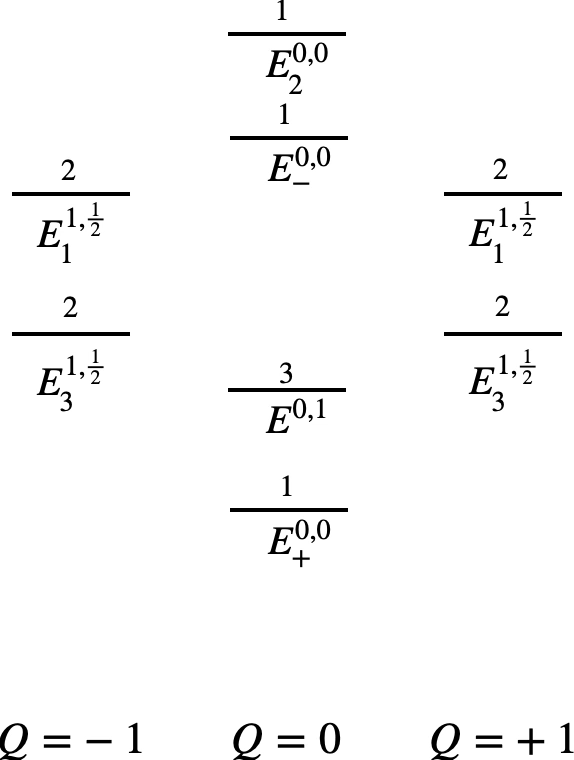
\includegraphics[width=0.6\linewidth,height=\textheight,keepaspectratio]{assets/splittingNLO.png}
\end{center}




\end{document}
